% no notes
\documentclass{beamer}
% notes and slides
%\documentclass[notes]{beamer}
% notes only
%\documentclass[notes=only]{beamer}
\usepackage{graphicx} % Allows including images
\usepackage{booktabs} % Allows the use of \toprule, \midrule and \bottomrule in tables
\usepackage{multirow}
\usepackage{multimedia}
\usepackage{circuitikz}
\usepackage{epigraph}
\usepackage{url}
\usepackage[framemethod=tikz]{mdframed}
\usepackage{tikz}
\usetikzlibrary{patterns,shapes.arrows}
\usetikzlibrary{positioning}
\usepackage[framemethod=tikz]{mdframed}
\usepackage{pgfplots}
\pgfplotsset{compat=newest}
\usepgfplotslibrary{groupplots,dateplot}
\usepackage{standalone}
\usepackage{adjustbox}
\usepackage{lmodern}
\usepackage{pgfplots}
\usepackage{amsmath}
\usepackage{amsthm}
\usepackage{multimedia}
\usepackage{standalone}
\usepackage{caption}
\usepackage{csquotes}

% python listings
% from https://tex.stackexchange.com/questions/83882/how-to-highlight-python-syntax-in-latex-listings-lstinputlistings-command
% Default fixed font does not support bold face
\DeclareFixedFont{\ttb}{T1}{txtt}{bx}{n}{12} % for bold
\DeclareFixedFont{\ttm}{T1}{txtt}{m}{n}{12}  % for normal

% Custom colors
\usepackage{color}
\definecolor{deepblue}{rgb}{0,0,0.5}
\definecolor{deepred}{rgb}{0.6,0,0}
\definecolor{deepgreen}{rgb}{0,0.5,0}

\usepackage{listings}

% Python style for highlighting
\newcommand\pythonstyle{\lstset{
language=Python,
basicstyle=\ttm,
morekeywords={self},              % Add keywords here
keywordstyle=\ttb\color{deepblue},
emph={MyClass,__init__},          % Custom highlighting
emphstyle=\ttb\color{deepred},    % Custom highlighting style
stringstyle=\color{deepgreen},
frame=tb,                         % Any extra options here
showstringspaces=false
}}


% Python environment
\lstnewenvironment{python}[1][]
{
\pythonstyle
\lstset{#1}
}
{}

% Python for external files
\newcommand\pythonexternal[2][]{{
\pythonstyle
\lstinputlisting[#1]{#2}}}

% Python for inline
\newcommand\pythoninline[1]{{\pythonstyle\lstinline!#1!}}

\definecolor{cyan}{RGB}{42,161,152}
\definecolor{violet}{RGB}{108,113,196}
\definecolor{red}{RGB}{220,50,47}

\PassOptionsToPackage{american}{babel} % change this to your language(s), main language last
% Spanish languages need extra options in order to work with this template
% \PassOptionsToPackage{spanish,es-lcroman}{babel}
\usepackage{babel}

\PassOptionsToPackage{%
  backend=biber,bibencoding=utf8, %instead of bibtex
  %backend=bibtex8,bibencoding=ascii,%
  language=auto,%
  style=numeric-comp,%
  %style=authoryear-comp, % Author 1999, 2010
  %bibstyle=authoryear,dashed=false, % dashed: substitute rep. author with ---
  style=alphabetic,
  sorting=nyt, % name, year, title
  maxbibnames=10, % default: 3, et al.
  %backref=true,%
  %natbib=true % natbib compatibility mode (\citep and \citet still work)
}{biblatex}
\usepackage{biblatex}

\usepackage{bm}

\newcommand{\bX}{\bm{X}}

\newcommand{\simplefig}[2]{\begin{figure}\includegraphics[width=#2\tw]{#1}\end{figure}}
\newcommand{\captionfig}[3]{\begin{figure}\includegraphics[width=#2\tw]{#1}\caption{#3}\end{figure}}
\newcommand{\cropfig}[3]{\begin{figure}\includegraphics[trim={#3},clip,width=#2\tw]{#1}\end{figure}}
\newcommand{\head}[1]{\vspace{3mm}\hrule\vspace{3mm}\structure{#1}\\}
\newcommand{\tw}{\textwidth}
\newcommand{\newl}{\hspace{1mm}\\}
\newcommand{\bmp}[1]{\begin{minipage}{#1}}
\newcommand{\bmpp}[2]{\begin{minipage}[#1]{#2}}
\newcommand{\emp}{\end{minipage}}
\newcommand{\cb}[1]{\left\{ {#1} \right\}}
\newcommand{\br}[1]{\left( {#1} \right)}
\newcommand{\sq}[1]{\left[ {#1} \right]}
\newcommand{\myemph}[1]{{\color{red}\emph{#1}}}

% Redefine the caption format to remove "Figure"
\captionsetup[figure]{labelformat=empty}

\newcommand{\referencefootnote}[1]{\setbeamertemplate{footline}[text line]{%%%
\parbox{0.9\paperwidth}{\vspace*{-23pt}\tiny{\textcolor{gray}{#1}}\hfill\scriptsize\insertframenumber}}}

\addbibresource{bib.bib}

\usetheme{metropolis}           % Use metropolis theme
\setbeamertemplate{caption}[default]
\title{Introduction to Convolutional Neural Networks}
\date{February 24, 2025}%{\today}
%\institute{High-Performance Computing and Analytics Lab}
%\author{Moritz Wolter}
\institute{Visual Computing Group, University of Bonn}
\author{Elena Trunz}

\titlegraphic{
\includegraphics[width=2.00cm]{UNI_Bonn_Logo_Standard_RZ.pdf}}
\begin{document}
    \maketitle

    \begin{frame}
    \frametitle{Overview} 
    \tableofcontents
    \end{frame}

    %\begin{frame}{Motivation \cite{goodfellow2016deep}}
        %\begin{itemize}
            %\item sparse interactions
            %\item parameter sharing
            %\item equivariant representations (i.e. with respect to translation)
            %\item efficiency
            %\item Train deeper networks.
        %\end{itemize}
        %\note{
            %Sparse interactions: From dense to block circulant matrix. \\
            %Parameter sharing: Use the same parameters for more than one job. \\
            %Equvariance: Translations of an input should not change the outcome.
        %}
    %\end{frame}
		
		\section{Why Convolution?}
		\begin{frame}{Invariance in the network structure}
	\begin{figure}
        \includestandalone[width=0.7\linewidth,height=1.5cm]{./figures/mnist_sequence}
      \end{figure}
			\begin{itemize}
		\item Consider the task of recognizing handwritten digits:
		\begin{itemize}
			\item Input image: set of pixel intensities
			\item Desired output: posterior probability over the ten digits
		\end{itemize} %\pause
		\item A system recognizing digits should be invariant to
		\begin{itemize}
			\item Translations
			\item Scaling
			\item (Small) rotations
			\item Some elastic deformations
		\end{itemize}
		\end{itemize}
	\end{frame}

	\begin{frame}{Fully connected network?}
	\begin{itemize}
		\item Given enough training data a fully connected network solves the task. %\pause
		\item However, we can do better: %\pause
		\begin{itemize}
			\item Pixels near to each other are more correlated to each other than pixels far apart. %\pause
			\item Local features which are useful in one region of the image are likely to be useful elsewhere as well, e.g. for detecting a translated object.
		\end{itemize}
		%\item In 1989 Yann LeCun proposed to build such invariance properties into the structure of a neural network. This is the basis for convolutional neural networks.
	\end{itemize} 
	\end{frame}

    \begin{frame}{The invention of convolutional neural networks}
        %Proposed in Yann le Cun's \cite{lecun1989handwritten}.
        In 1989 Yann LeCun proposed to build invariance properties into the structure of a neural network. 
				\begin{figure}%
				\centering
				%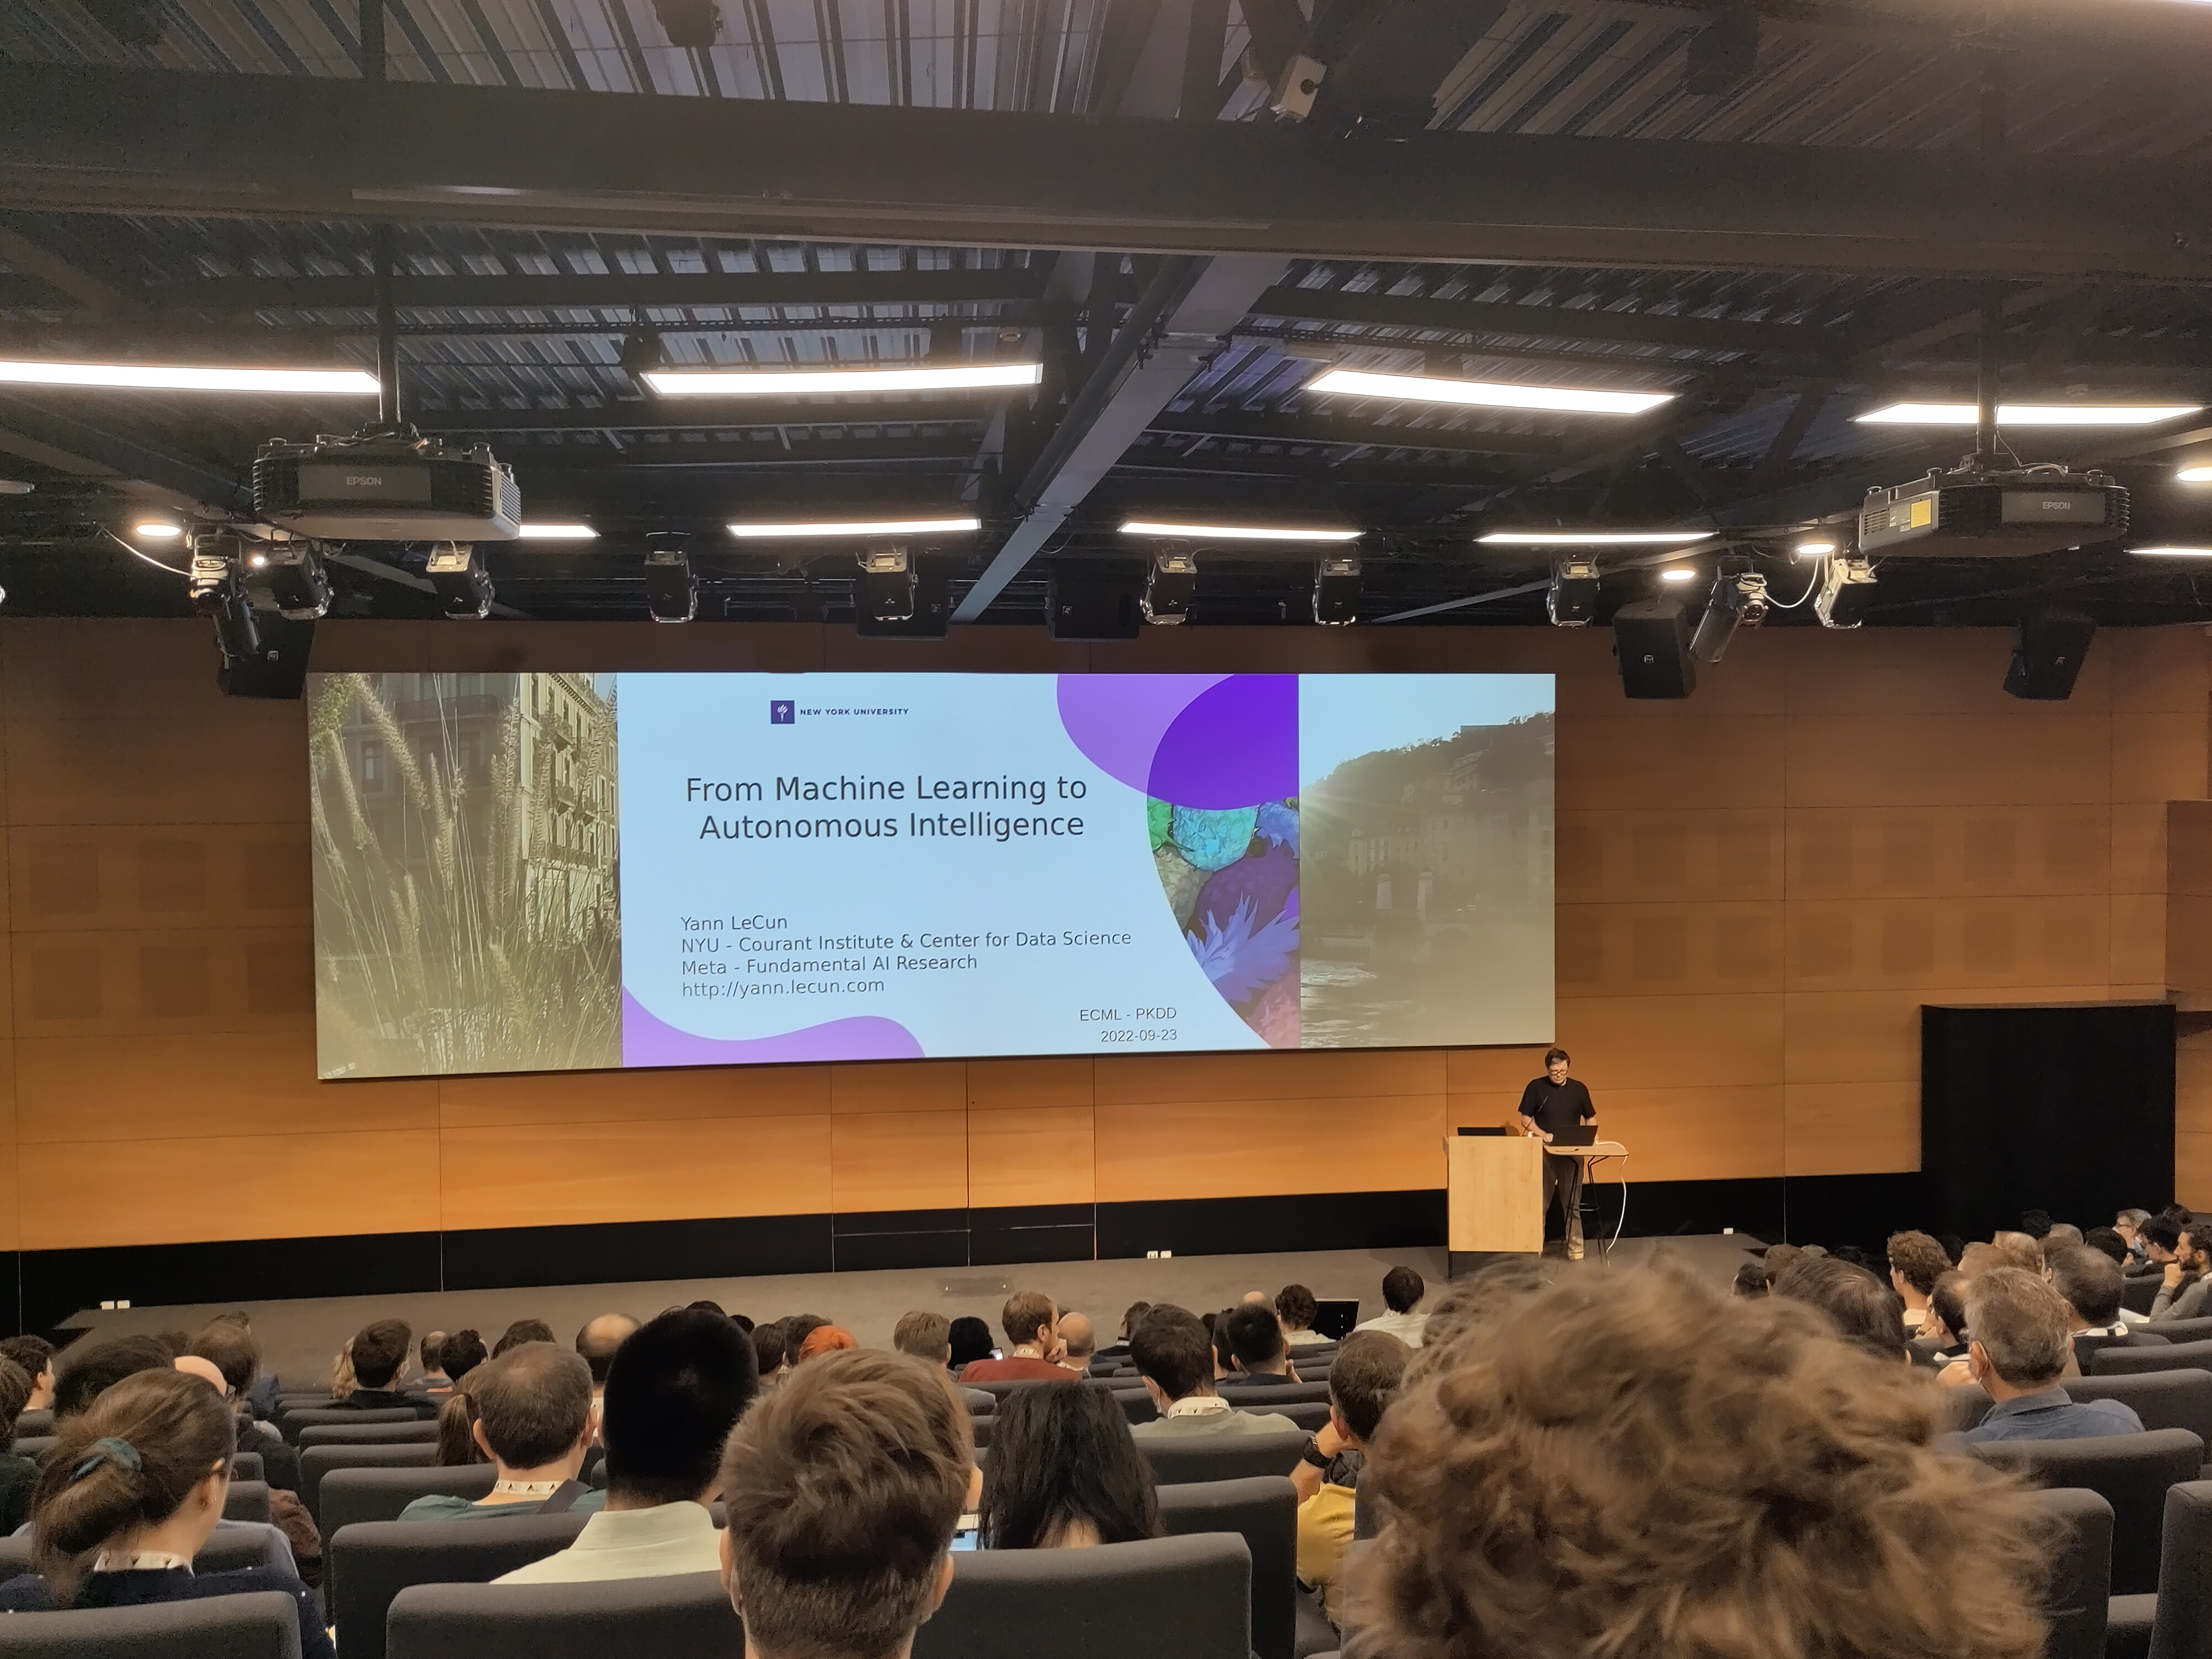
\includegraphics[width=.6\linewidth]{figures/IMG_20220923_090433.jpg}
				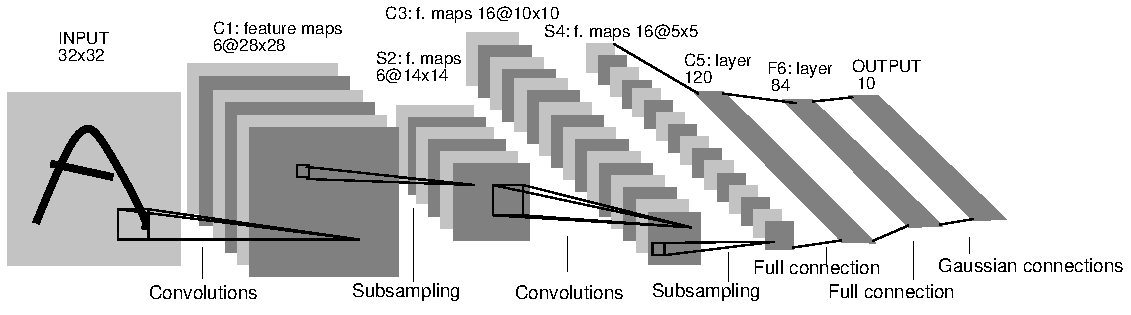
\includegraphics[width=1.0\linewidth]{figures/lenet5.pdf}
				\end{figure}   
				\note{This is the basis for convolutional neural networks.}
    \end{frame}
		
    \section{Convolution operation in machine learning}

    %\begin{frame}{Defining convolution}
			%For two one-dimensional signals $x \in \mathbb{R}^T$
        %and $k \in \mathbb{R}^T$, convolution is defined as
        %\begin{align}
            %s(t) = (x * k)(t) = \sum_{a=0}^{T} x(a)k(t - a),
        %\end{align}
        %for numbers $t,a$. Possible $t$ will depend on signal length and padding. \\
        %In 2D, we require a kernel matrix $K \in \mathbb{R}^{O,P}$ and a image matrix
        %$I \in \mathbb{K}^{N,M}$
        %\begin{align}
            %S(i,j) = (K * I)(i,j) = \sum_m^M \sum_n^N I(i-m, j-n)K(n,m)
        %\end{align}
        %Again not just any $i,j$ will do. We will see what this means in a minute.
    %\end{frame}
		
		 \begin{frame}{Defining discrete convolution}
		\begin{itemize}
			\item For two one-dimensional signals $x \in \mathbb{R}^T$
        and $k \in \mathbb{R}^T$, convolution is defined as
        \begin{align}
            s(t) = (x * k)(t) = \sum_{m=0}^{T} x(m)k(t - m),
        \end{align}
				where $t$ denote the position in the output sequence. %\pause
        \item In 2D, we require a kernel matrix $K \in \mathbb{R}^{O,P}$ and a image matrix
        $I \in \mathbb{K}^{N,M}$
        \begin{align}
            S(i,j) = (K * I)(i,j) = \sum_m^M \sum_n^N I(i-m, j-n)K(n,m)
        \end{align}
				where $(i,j)$ denote the position in the output image.
				\end{itemize}
				\note{$m$ and $n$ are indices that iterate over the elements of the input and the kernel.}
    \end{frame}


    \begin{frame}{Defining cross-correlation}
        \begin{itemize}
					\item Cross-correlation is convolution without flipping the kernel: % \cite{goodfellow2016deep}
        \begin{align}
            S(i,j) = (K*I)(i,j) = \sum_m^M \sum_n^N I(i+m, j+n)K(m,n)
        \end{align}
        \item Many machine-learning libraries implement cross-correlation and
        call it convolution. 
				\item In this course we will follow their example.
				\end{itemize}
    \note{
        A convolution example on the board: 
        \begin{align}
            \mathbf{I} = \begin{pmatrix}
                1 & 3 & -1 \\
                2 & 1 &  0 \\
                0 & 2 & -1 \\
            \end{pmatrix},
            \mathbf{K} = \begin{pmatrix}
                1 & 0 \\
                2 & -1 \\
            \end{pmatrix}
        \end{align}
        Computing $\mathbf{I}*\mathbf{K}$:
        \begin{align}
            \mathbf{I}*\mathbf{K} &= \begin{pmatrix}
                1\cdot 1 + 3\cdot 0 + 2\cdot 2 + 1\cdot (-1) & 3\cdot 1 + (-1)\cdot 0 + 1\cdot 2 + 0\cdot (-1) \\
                2\cdot 1 + 1\cdot 0 + 0\cdot 2 + 2\cdot (-1) & 1\cdot 1 + 0\cdot 0 + 2\cdot 2 + (-1)\cdot (-1)  
            \end{pmatrix} \\
            &= \begin{pmatrix}
                4 & 5 \\
                0 & 6
            \end{pmatrix}
        \end{align}
    }
    \end{frame}

    \begin{frame}{Convolution}
        \begin{figure}
            \centering
            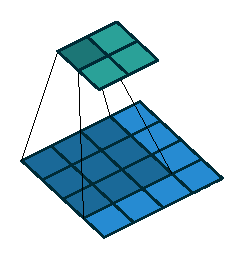
\includegraphics[scale=0.7]{./figures/no_padding_no_strides_00.pdf}
            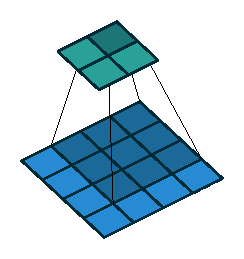
\includegraphics[scale=0.7]{./figures/no_padding_no_strides_01.pdf} \\
            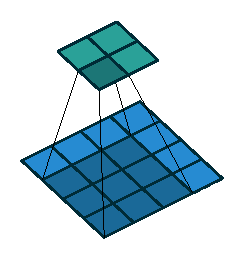
\includegraphics[scale=0.7]{./figures/no_padding_no_strides_02.pdf}
            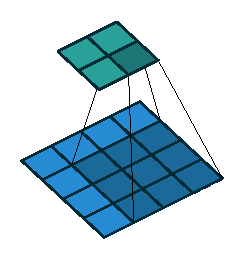
\includegraphics[scale=0.7]{./figures/no_padding_no_strides_03.pdf}
            \caption{Illustration of the convolution operation \cite{dumoulin2016guide}.}
        \end{figure}
    \end{frame}
		
		\begin{frame}{Advantages of convolutions}
	The convolution operation allows us to do this for inputs of varying sizes in a convenient way, and affords advantages of  %\pause 
	\begin{enumerate}
	\item local receptive fields (sparse connectivity limited in range vs. fully connected) %\pause 
	\item parameter sharing (allows for detection of same features all over the image) %\pause 
	\item equivariant representations and subsampling (reduces information hierarchically)
	\end{enumerate}
	\end{frame}


	\begin{frame}{Sparse connectivity and interaction}
	\footnotesize
	\begin{itemize}
		\item In CNNs, the kernel or filter is often much smaller than the input size.  This allows us to process images of varying sizes.  For an input image of millions of pixels we can still detect meaningful features which are local, such as edges. 
		\item A small kernel does not mean that the area of interaction is limited.  For a deep network, the units may \emph{indirectly} interact with a larger portion of the input as information propagates up the layers:
	\captionfig{figures/dl9_4}{0.35}{\footnotesize Unit $g_3$ indirectly interacts with the whole input \cite{goodfellow2016deep}}
	\end{itemize}
	\end{frame}

{ \referencefootnote{Image was taken from \cite{goodfellow2016deep}}
	\begin{frame}{Parameter sharing}
	\footnotesize
	\begin{itemize}
		\item Standard feed-forward network has unit-specific weights. %\pause
		\item Each weight is used only once when computing the activations for subsequent layers. %\pause
		\item In a CNN, the weights of each kernel is applied to every position of the input. %\pause
		\item This \emph{parameter sharing} reduces the amount of storage per model.
		%\captionfig{figures/dl9_5}{0.3}{9.5 from Goodfellow}
		\begin{figure}
					\center
					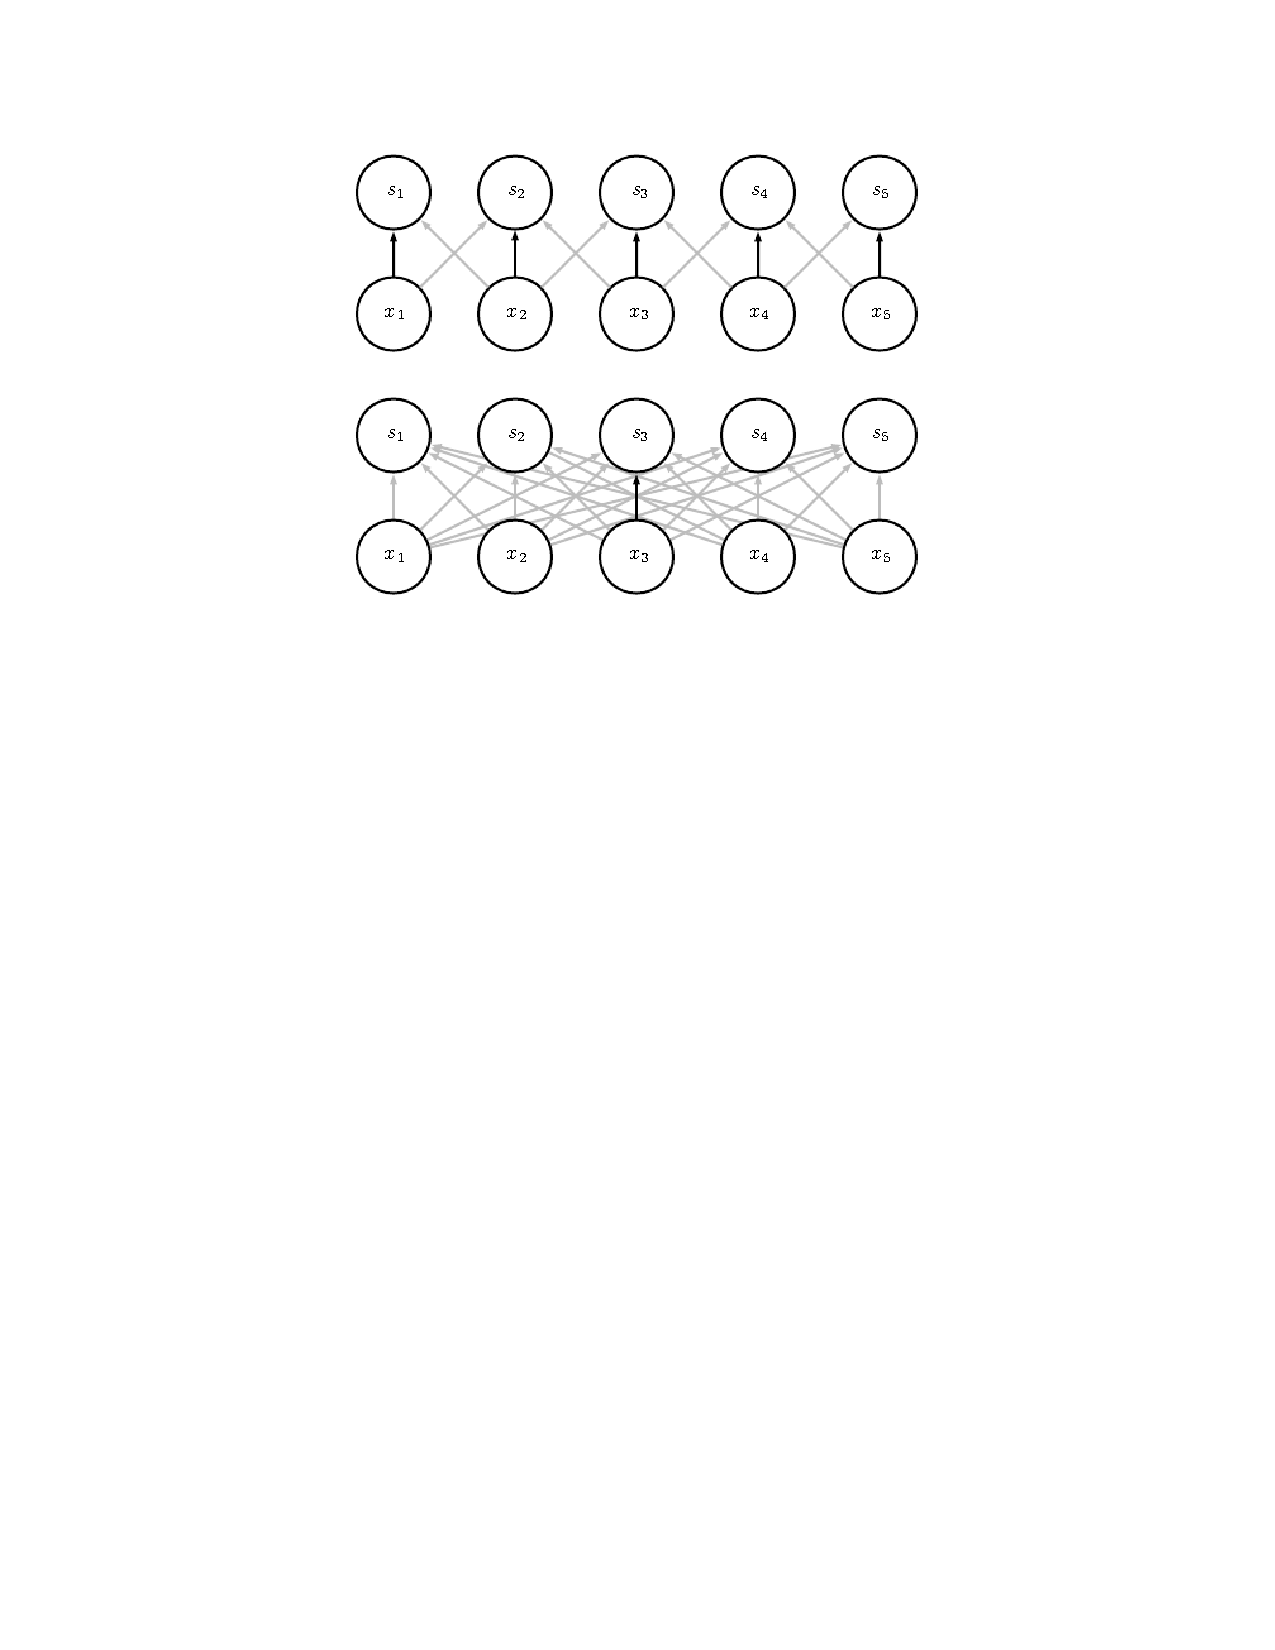
\includegraphics[scale=.4]{figures/dl9_5.pdf} 
					%\caption{}
					\end{figure}
	\end{itemize}
	\end{frame}
	}
	\note{The black arrows show connections that use a particular parameter set in two different models.  If we were to share parameters, then the single parameter (set) is used at all the input locations.  But if were to have a fully-connected layer, then this set of parameters would be used only once, which is shown in the bottom figure.}


	\begin{frame}{Translation equivariance}
	\begin{itemize}
		\item An \emph{equivariant} function is one where for some given change in the input, the output changes in the same way.%\pause 
		\item With images, convolution creates a 2-D map of where certain features appear in the input. If we move the object in the input, its representation will move the same amount in the output.
	\end{itemize}
	\end{frame}
	\note{equivariance is useful for finding repeating patterns, e.g. line detection;}

	\begin{frame}{Strided convolution}
	\begin{itemize}
		\item To save computational expense, we can skip over some positions of the kernel, i.e. not extract our feature response as finely.
	\begin{figure}
            \centering
            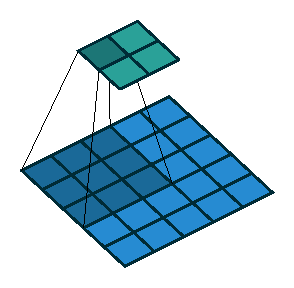
\includegraphics[width=0.2\linewidth]{figures/no_padding_strides_00.pdf}
            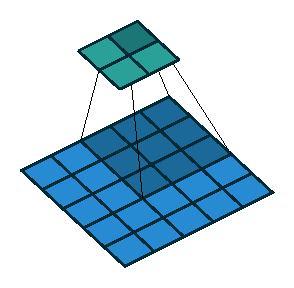
\includegraphics[width=0.2\linewidth]{figures/no_padding_strides_01.pdf} \\
            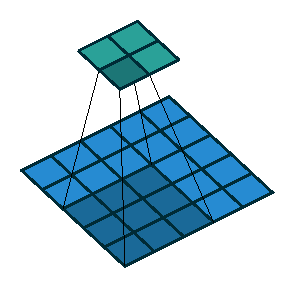
\includegraphics[width=0.2\linewidth]{figures/no_padding_strides_02.pdf}
            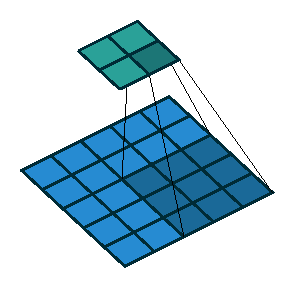
\includegraphics[width=0.2\linewidth]{figures/no_padding_strides_03.pdf}
            \caption{Stride two convolutions \cite{dumoulin2016guide}.}
        \end{figure}
				\item[$\rightarrow$] Down-sampling
		\end{itemize}
	\end{frame}
	
		{ \referencefootnote{Image was taken from \cite{goodfellow2016deep}}
    \begin{frame}{Padded convolution}
		\begin{itemize}
			\item We can control the size of convolution inputs and outputs through padding. 
			\item Without padding, the spatial extent of the network would shrink, with the rate of shrinking directly proportional to the size of the filter or kernel.  
        \begin{figure}
            \centering
            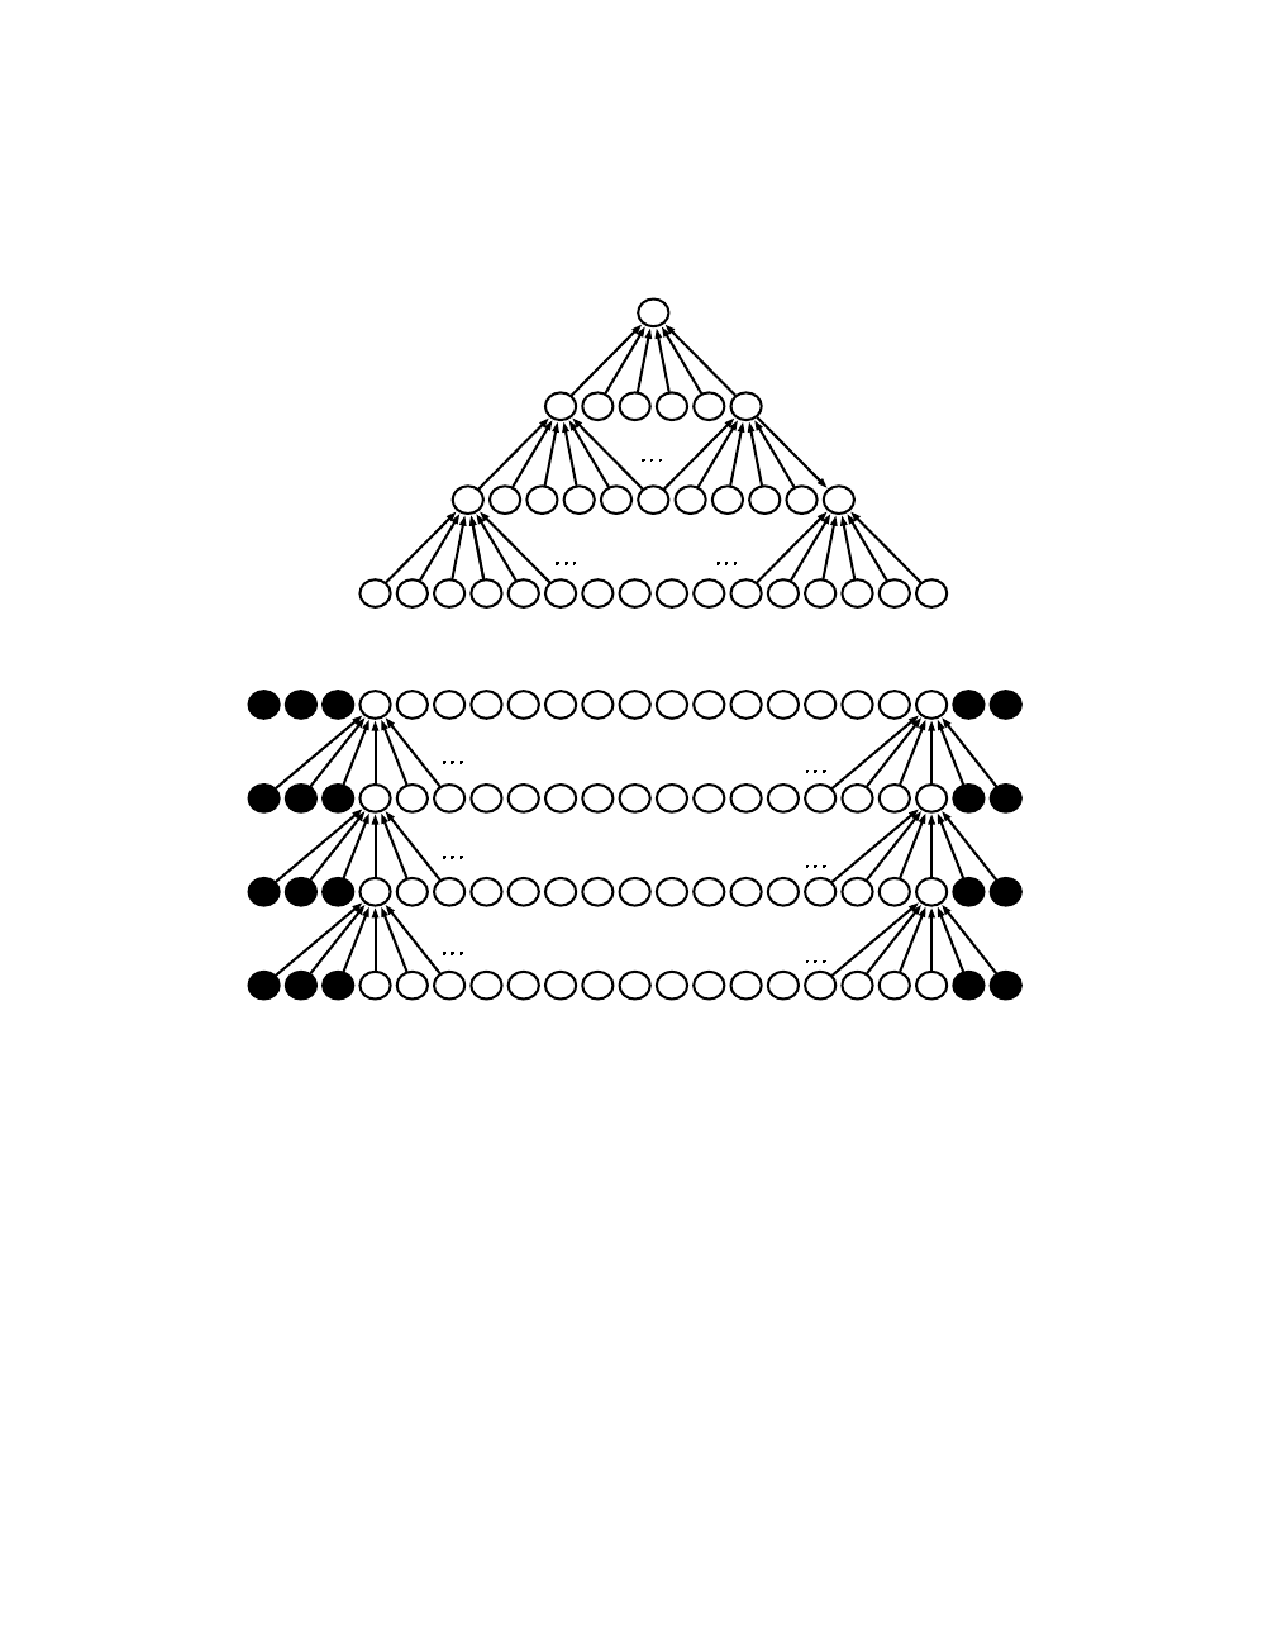
\includegraphics[width=0.45\linewidth]{figures/dl9_13.pdf}
            %\caption{}
        \end{figure}
				\end{itemize}
    \end{frame}
		}

    %\begin{frame}{Visualization of padded convolution}
        %\begin{figure}
            %\centering
            %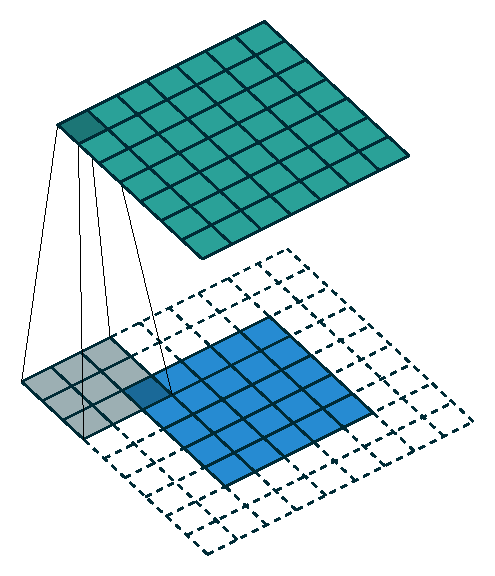
\includegraphics[width=0.25\linewidth]{./figures/full_padding_no_strides_00.pdf}
            %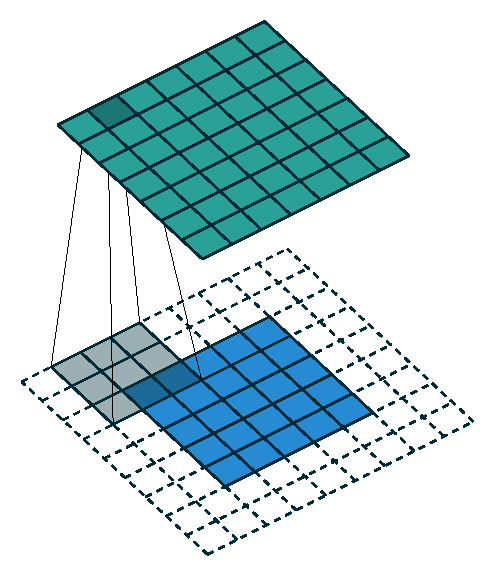
\includegraphics[width=0.25\linewidth]{./figures/full_padding_no_strides_01.pdf} \\
            %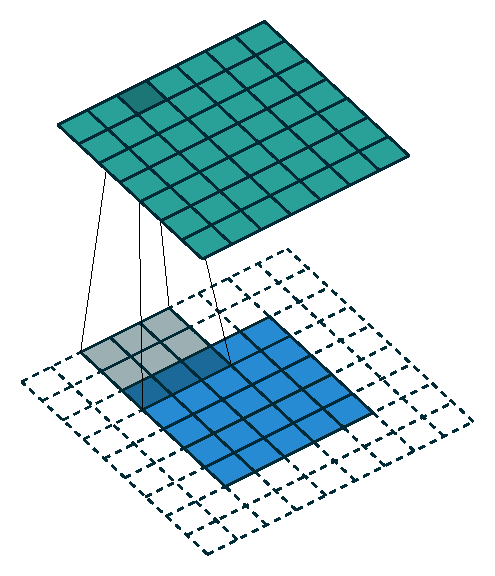
\includegraphics[width=0.25\linewidth]{./figures/full_padding_no_strides_02.pdf}
            %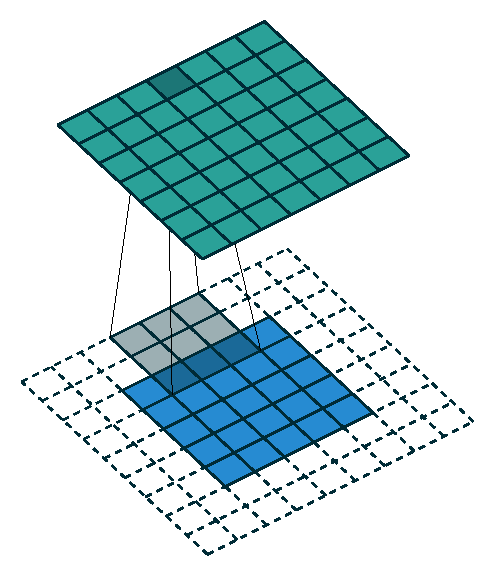
\includegraphics[width=0.25\linewidth]{./figures/full_padding_no_strides_03.pdf}
            %\caption{Fully padded convolutions with unit strides \cite{dumoulin2016guide}.}
        %\end{figure}
    %\end{frame}

    \begin{frame}{Summary}
        \begin{itemize}
            \item The convolution operation slides convolution kernels over an image.
            \item Padding avoids losing pixels on the side.
            \item Strided convolutions downsample the input.
            \item Moving in steps of two pixels, for example, cuts the resolution in half.
        \end{itemize}
    \end{frame}

    \section{Understanding convolution}

    \begin{frame}{Getting computers to find Waldo}
        \begin{figure}
            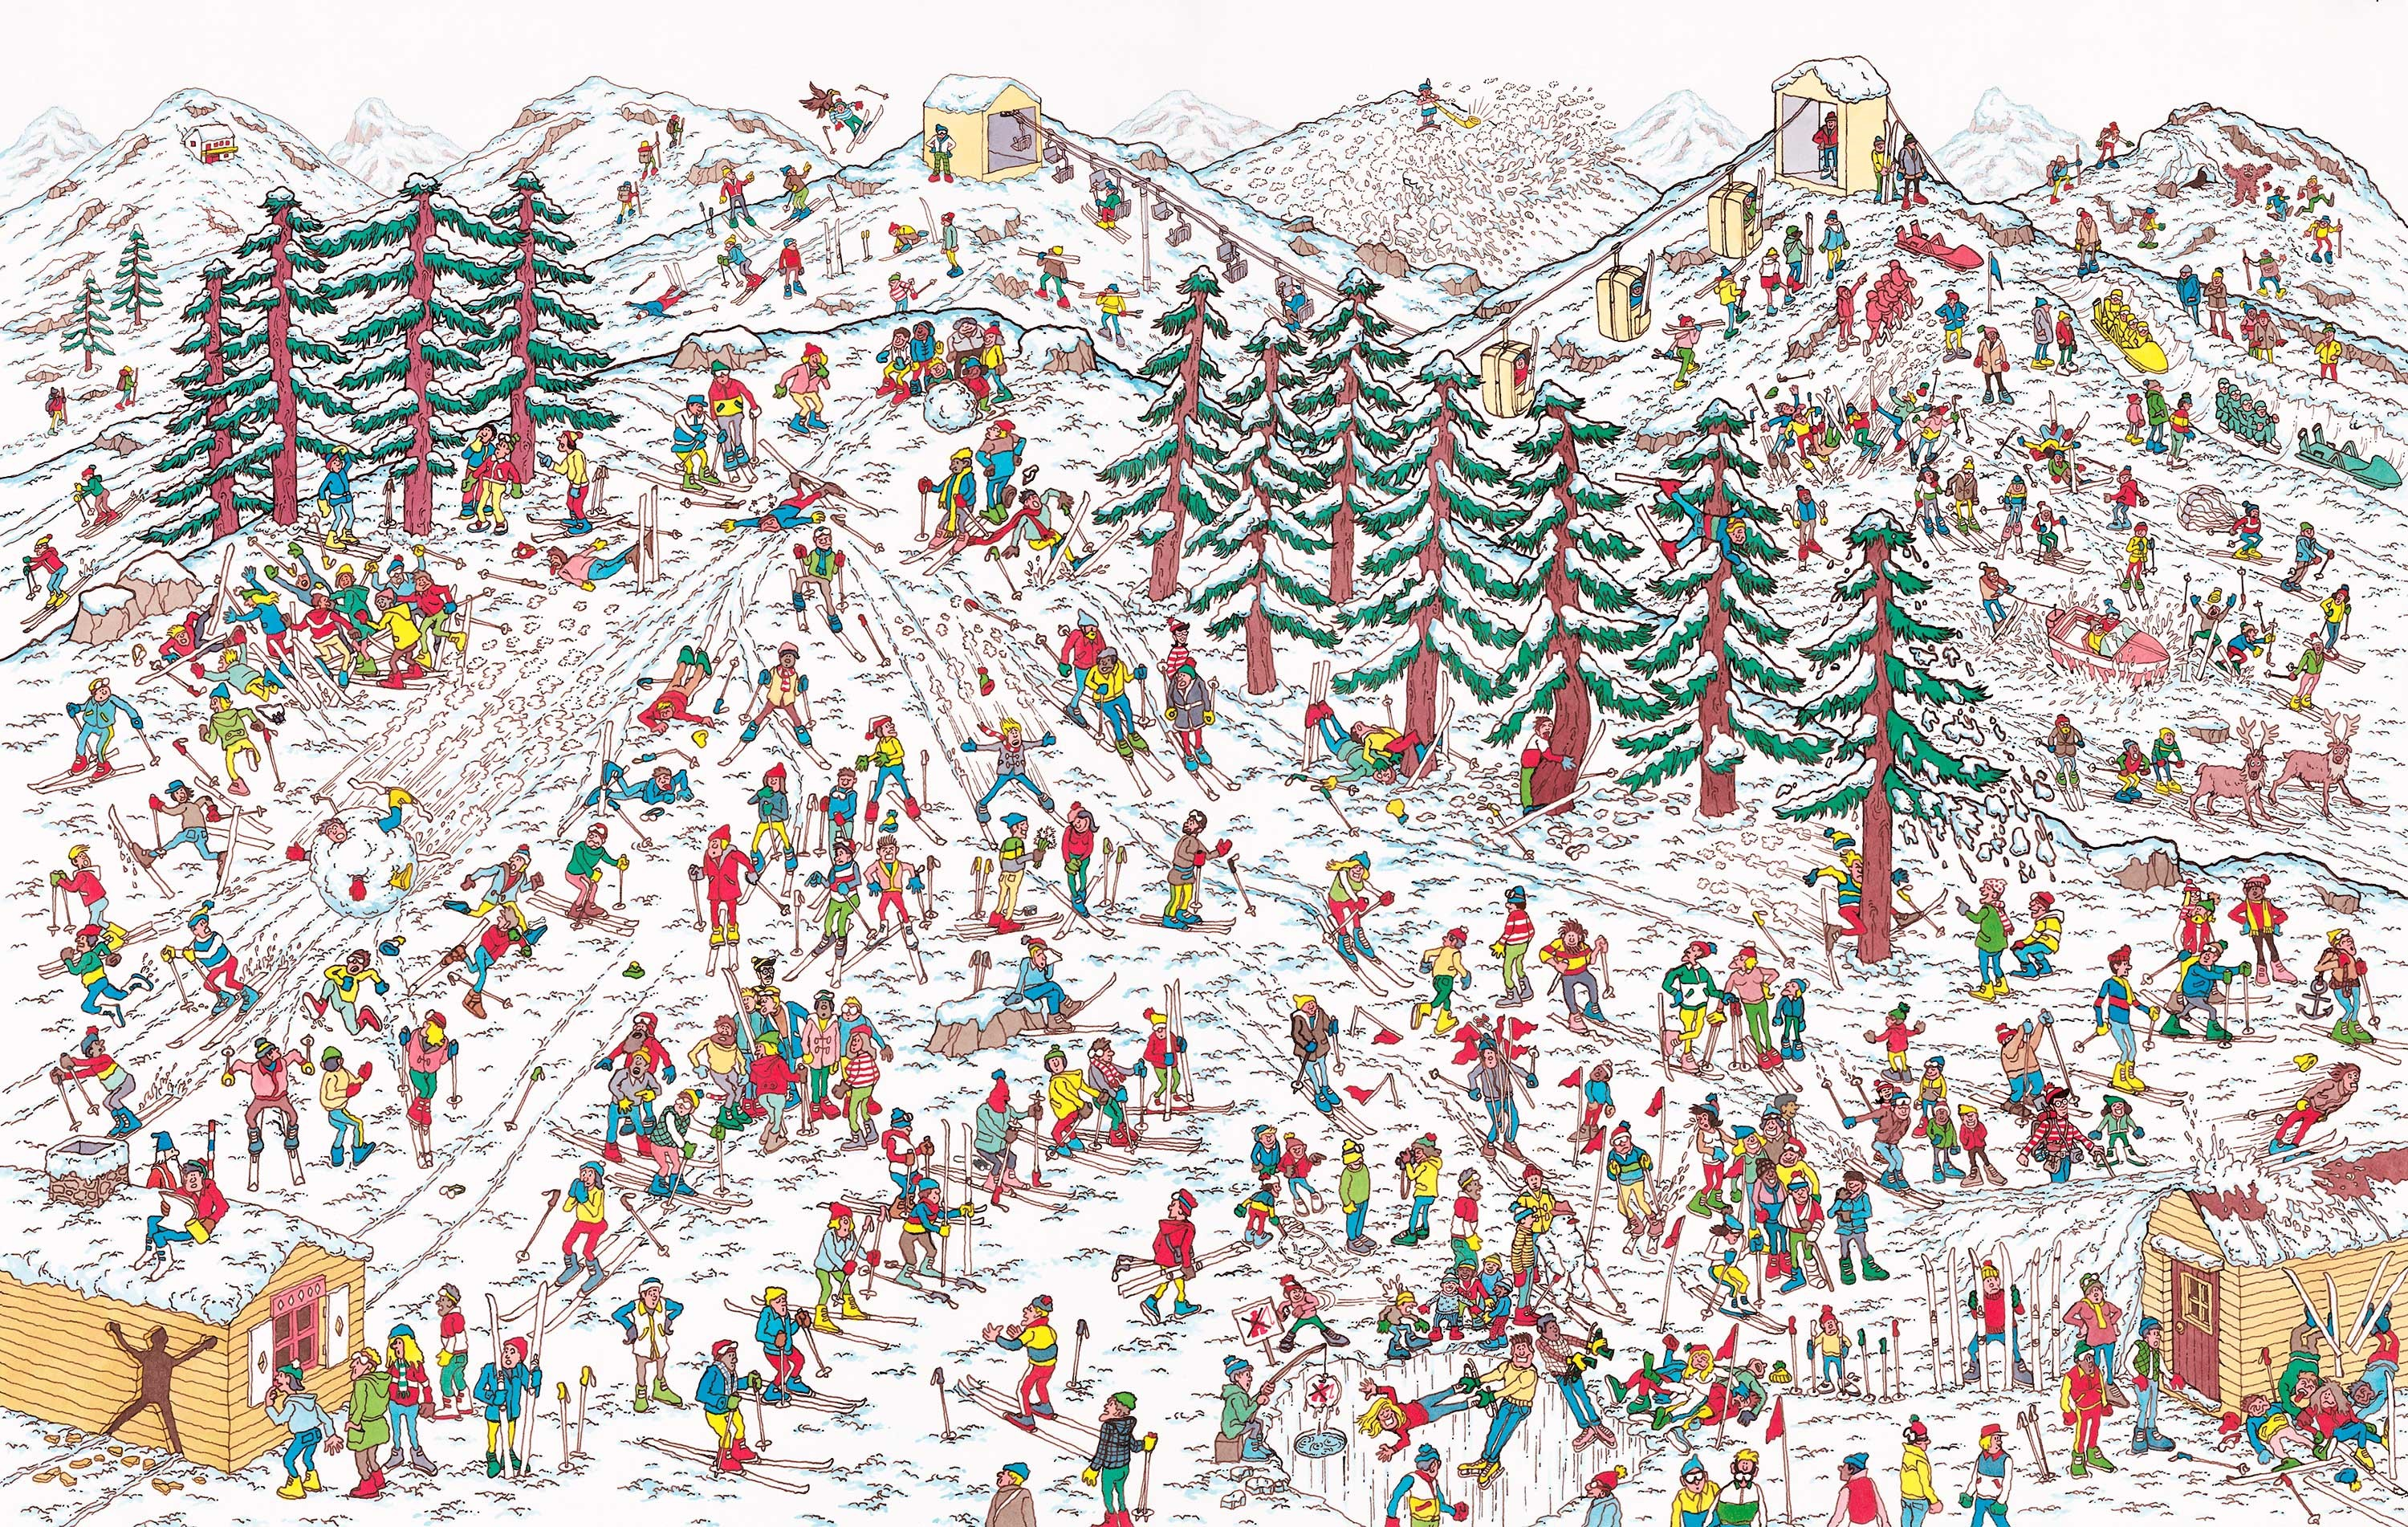
\includegraphics[scale=0.1]{./python/waldo_snow.jpg}
            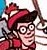
\includegraphics{./python/waldo_small.jpg}
        \end{figure}
    \end{frame}

    \begin{frame}{Finding Waldo via cross-correlation.}
        \begin{figure}
        \centering
        \includestandalone[scale=1]{./figures/corr_plot}
        %\caption{}
        \end{figure}
    \end{frame}

    \begin{frame}{Summary}
        \begin{itemize}
            \item Cross-correlation is called convolution in the machine learning literature.
            \item Patterns can be located in signals via cross-correlation.
        \end{itemize}
    \end{frame}

    \section{Convolutional neural networks}
    \begin{frame}{Motivating convolutional neural networks (CNN)}
        \begin{itemize}
            \item Fixed filters work if we are looking for a very specific waldo.
            \item In other cases, we need a better solution.
            \item Convolutional neural networks rely on filter optimization via back-propagation.
            \item Filter optimization turns CNNs into very versatile tools!
        \end{itemize}
    \end{frame}
	
	\begin{frame}{Multiple filters / kernels}
	\begin{itemize}
		\item In the context of CNNs, we refer to convolution not in the strict mathematical sense, but an operation that applies many convolutions in parallel.
		\item Convolution with a single kernel extracts only one kind of feature (at many spatial locations).
		\item For each layer, however, we are interested in extracting many kinds of features (at many spatial locations). 
	\end{itemize}
	\end{frame}

    \begin{frame}{Multichannel convolution}
        \begin{figure}
            \includestandalone[width=.8\linewidth]{./figures/cnn_channels}
            \caption{The plot shows a convolution
            computation using a $3x2x3x3$ kernel on a $2x5x5$ input.
            The kernel pairs convolve with the input, producing $3x3$ results.
            $+$ adds the two channels for each of the three tensors.
            Finally, everything is stacked. Inspired by \cite[page 9]{dumoulin2016guide}. }
        \end{figure}
        \note{
            On the board:
            Explain the effect of the input and output shapes. \\
            I.e.: \\
                Kernel $(O,I,H,W)$:  Out-Channels, In-Channels, Height, Width \\
                Image  $(N,C,H,W)$: Batch-Size, Channels, Height, Width \\
                Results in: \\
                Result $(N,O, H_n, W_n)$ 
        }
    \end{frame}

    %\begin{frame}{Computing the output shape of a CNN layer}
        %One can determine the output shape for each dimension individually.
        %Without zero padding and a stride size of one,
        %\begin{align}
            %o = (i-k) + 1
        %\end{align}
        %can be used to compute the output size. $i$ denotes the input size,
        %and $k$ is the kernel size. \cite{dumoulin2016guide} covers all cases which appear in practice.
    %\end{frame}

		\begin{frame}{Calculating the output size}
		\[
		W_{out} = (W_{in}-K+2P)/S+1
		\]
	\begin{itemize}
		\item $W_{in}$: input size (width or height)
		\item $W_{out}$: output size (width or height)
		 \item  $K$: kernel size
			\item $P$: padding
			\item $S$: stride
	\end{itemize}
		\end{frame}
	
    \begin{frame}{Image to column and the forward pass}
        We already know how to train dense network layers using matrix multiplication.
        Training a CNN the same way requires restructuring the image to express convolution as matrix multiplication,
        \begin{align}
            \overline{\mathbf{h}} &= \mathbf{K}_f \mathbf{v}_I  + \mathbf{b}, \\ 
            \mathbf{h}_f &= f(\overline{\mathbf{h}}).
        \end{align}
        $\mathbf{v}_I \in \mathbb{R}$ denotes the restructured image input. $\mathbf{K}_f \in \mathbb{R}^{k_o, k_i \cdot k_h \cdot k_w}$ the flattened restructured kernel.
        $o,i,h,w$ denote the output, input, height, and width dimensions, respectively.
        \note{
            im2col demonstrate on the board:
            Idea: collect the image convolution patches in the columns of a matrix. Use python indexing to set it up.
            For a $3 \times 3$ matrix and a $2 \times 2$ kernel without padding this would lead to the index matrices: 
            \begin{align}
                \begin{pmatrix}
                    0 & 1 & 2 \\
                    3 & 4 & 5 \\
                    6 & 7 & 8 \\
                \end{pmatrix}
                \rightarrow
                \begin{pmatrix}
                0 & 1 & 3 & 4 \\
                1 & 2 & 4 & 5 \\
                3 & 4 & 6 & 7 \\
                4 & 5 & 7 & 8
                \end{pmatrix}
            \end{align}
        }
    \end{frame}

    \begin{frame}{The backward pass}
        We apply the rules for dense layers to the restructured convolutional layer data,
        \begin{align} 
            \delta \mathbf{K}_f &= [f'(\overline{\mathbf{h}}) \odot \triangle]_f \mathbf{v}^T_I,  &  
            \delta \mathbf{b} &= f'(\overline{\mathbf{h}}) \odot \triangle,   \\  
            \delta \mathbf{x} &= \big(\mathbf{K}_f^T [f'(\overline{\mathbf{h}}) \odot \triangle]_f \big)_{I^{-1}}.
        \end{align}
        With $I$ and $I^{-1}$ denoting the \texttt{im2col} and \texttt{col2im} operations.
        All major deep learning frameworks have both operations built in.
    \end{frame}
		
			\begin{frame}{A CNN layer}
	A typical layer of a CNN has three stages:
	\begin{enumerate}
	\item convolution operation %\pause 
	\item a non-linear activation, e.g. rectified linear unit %\pause
	\item a pooling function which replaces the output at a certain location with some summary statistic of nearby outputs
	\end{enumerate}
	\end{frame}

{ \referencefootnote{\href{http://cs231n.github.io/assets/cnn/maxpool.jpeg}{\underline{Image link}}}
	\begin{frame}{Max pooling}
	\footnotesize
	\begin{itemize}
		\item One of the most common summary statistics used is \emph{max-pooling}.
	\begin{figure}
            \centering
            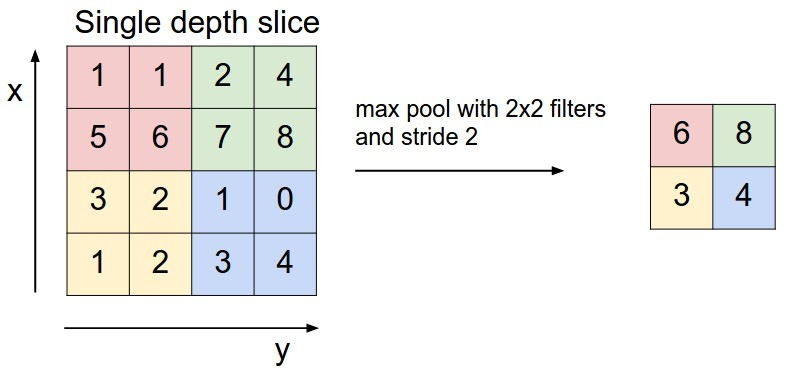
\includegraphics[width=0.6\linewidth]{figures/maxpool.jpeg}
            %\caption{}
        \end{figure}
	\item Max pooling affords some extra tolerance to spatial shifts.%\pause
	\item For many tasks, pooling is an essential step which allows handling input images of varying sizes.  
	\item This can be handled by varying the size of an offset between pooling regions, so that a subsequent classification layer always receives the same number of pooled statistics, regardless of input size.
	\end{itemize}
	\end{frame}
	}
	\note{Pooling helps to make the representation become approximately invariant to small translations of the input.  Invariance to local translation is very useful if we care about whether some feature is present rather than exactly where it is.  For instance, when detecting a face, it is not important to know the exact location of the left eye, rather than just known that there is an eye present on the left side of the face and there is an eye present on the right side of the face.}

    \begin{frame}{The classifier at the end}
        \begin{figure}%
				\centering
				%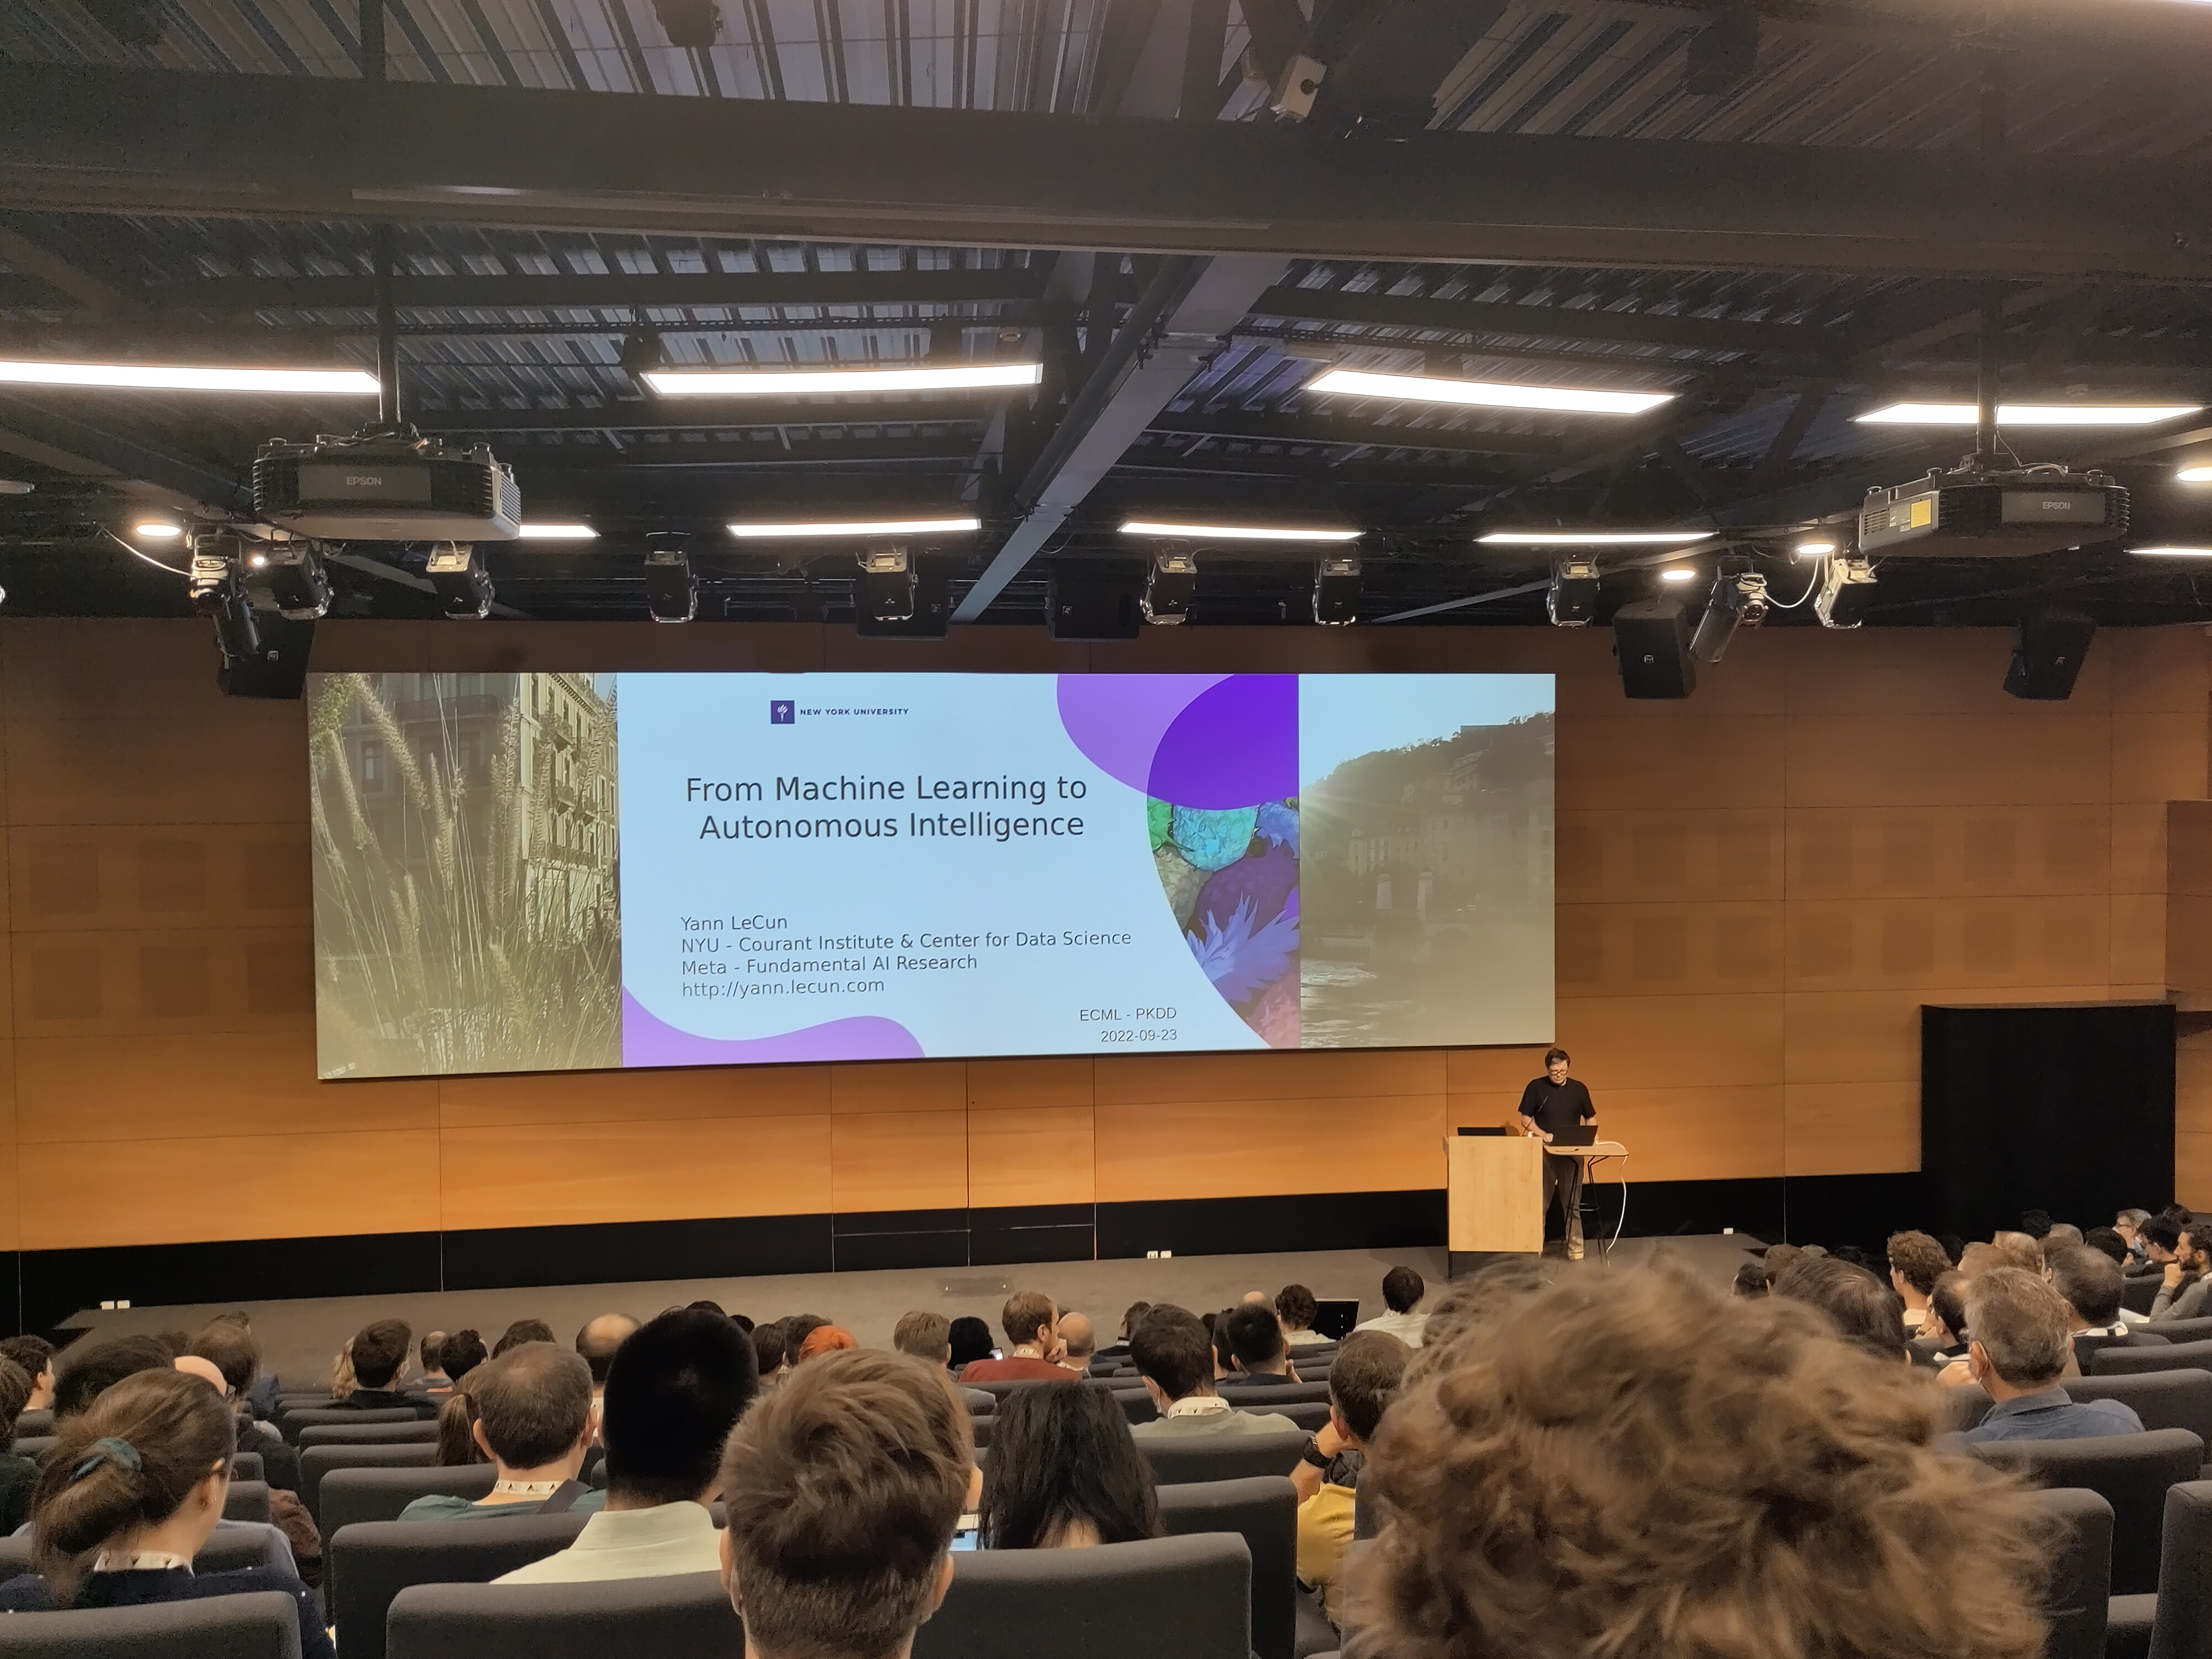
\includegraphics[width=.6\linewidth]{figures/IMG_20220923_090433.jpg}
				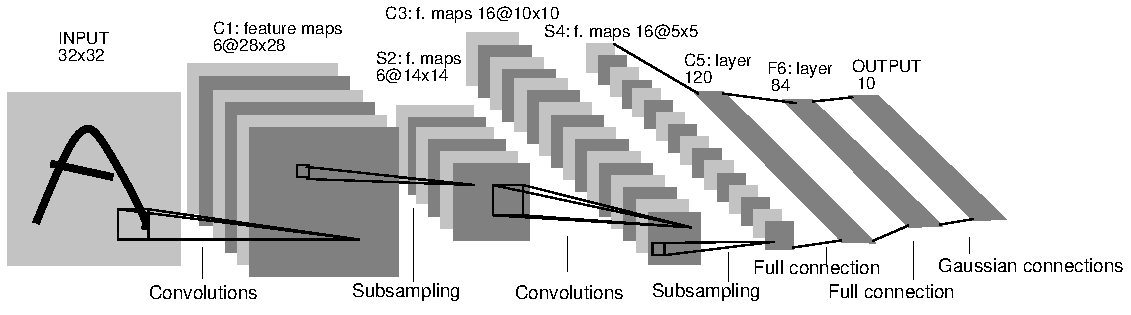
\includegraphics[width=1.0\linewidth]{figures/lenet5.pdf}
        \caption{The LeNet5-architecture\cite{lecun1989handwritten}.}
        \end{figure}
    \end{frame}

    %\begin{frame}{The shifting input problem}
        %\begin{itemize}
            %\item With the tools we have seen, shifting an input also shifts the CNN output before the dense classifier.
            %\item Shifting the input would shift the input in front of the final dense-classifier neurons.
            %\item We want invariance to translation.
        %\end{itemize}
    %\end{frame}
%
%
    %\begin{frame}{Pooling}
        %Max pooling layers choose maximum values in predefined regions.
        %Two by two max pooling, for example, picks the maximum in neighboring areas of four pixels.
        %If an input is shifted by two pixels, the result will remain the same!
        %Pooling layers are used repeatedly for a cumulative effect.
        %\note{
            %$\rightarrow $ Draw the effect of max pooling on the board.
        %}
    %\end{frame}

    \begin{frame}{MNIST}
        \begin{figure}
            \includestandalone[height=1cm, width=6cm]{./figures/mnist_sequence}
            \caption{Sample digits from the MNIST-database.}
        \end{figure}
        \begin{figure}
            \includestandalone[scale=.6]{./figures/cnn_mnist}
            \caption{Mean convergence of two-layer CNN with a dense classifier.}
        \end{figure}
    \end{frame}

	\section{Deep convolutional neural networks}
	
    \begin{frame}{Deeper models perform better}
        \begin{figure}
            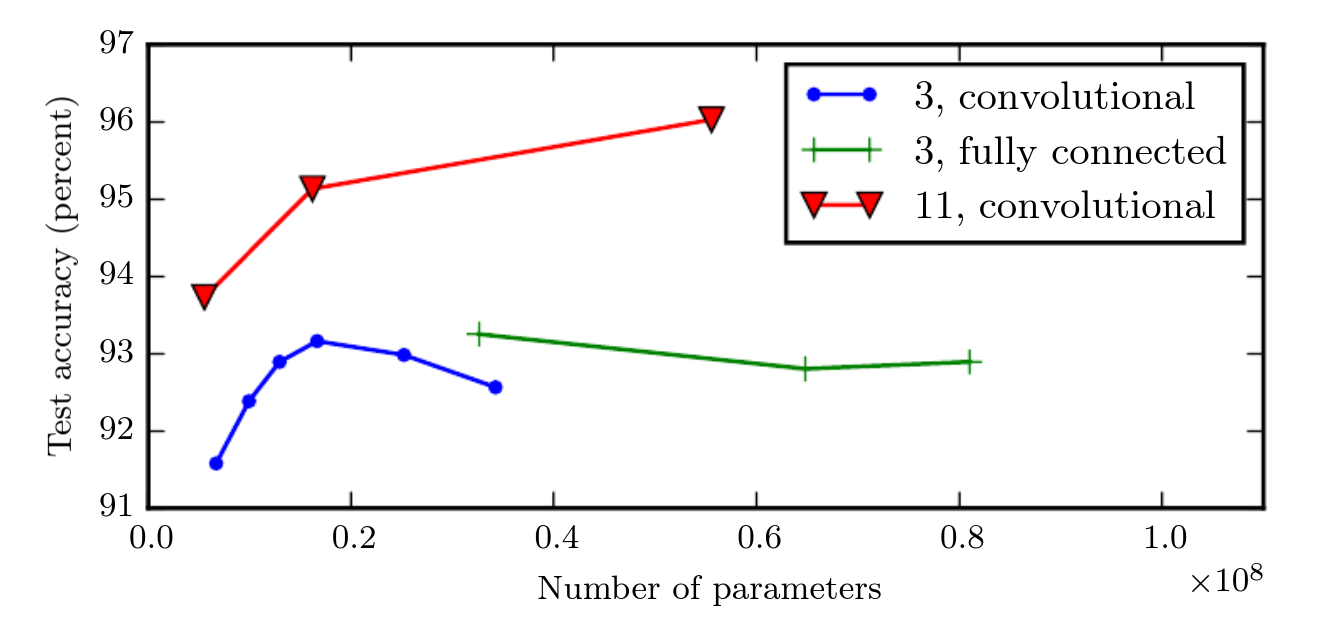
\includegraphics[width=0.8\linewidth]{figures/deep_cnn.png}
            \caption{Comparing deep networks with and without convolutional structures on the Google-Street view dataset
                \cite[page 199]{goodfellow2016deep}.}
        \end{figure}
        \note{ \cite{goodfellow2016deep} tells us: \\ 
        Effect of number of parameters. Deeper models tend to perform better.
        This is not merely because the model is larger. This experiment from Goodfellow et al.
        (2014d) shows that increasing the number of parameters in layers of convolutional networks
        without increasing their depth is not nearly as effective at increasing test set performance,
        as illustrated in this figure.}
    \end{frame}

	\begin{frame}{Boom of CNNs}
	The use of CNNs for visual recognition really took off in 2012, where the winning entry of the ImageNet object recognition challenge was a CNN.
	\cropfig{figures/pg_0023.pdf}{0.8}{0cm 1.5cm 0cm 0cm}
	\end{frame}
	
	{ \referencefootnote{\href{http://ai.stanford.edu/~olga/slides/berkeley_ilsvrc_2014.pdf}{Slide from \underline{here}.}}
		\begin{frame}{Modern CNNs}
		\begin{figure}
            \centering
            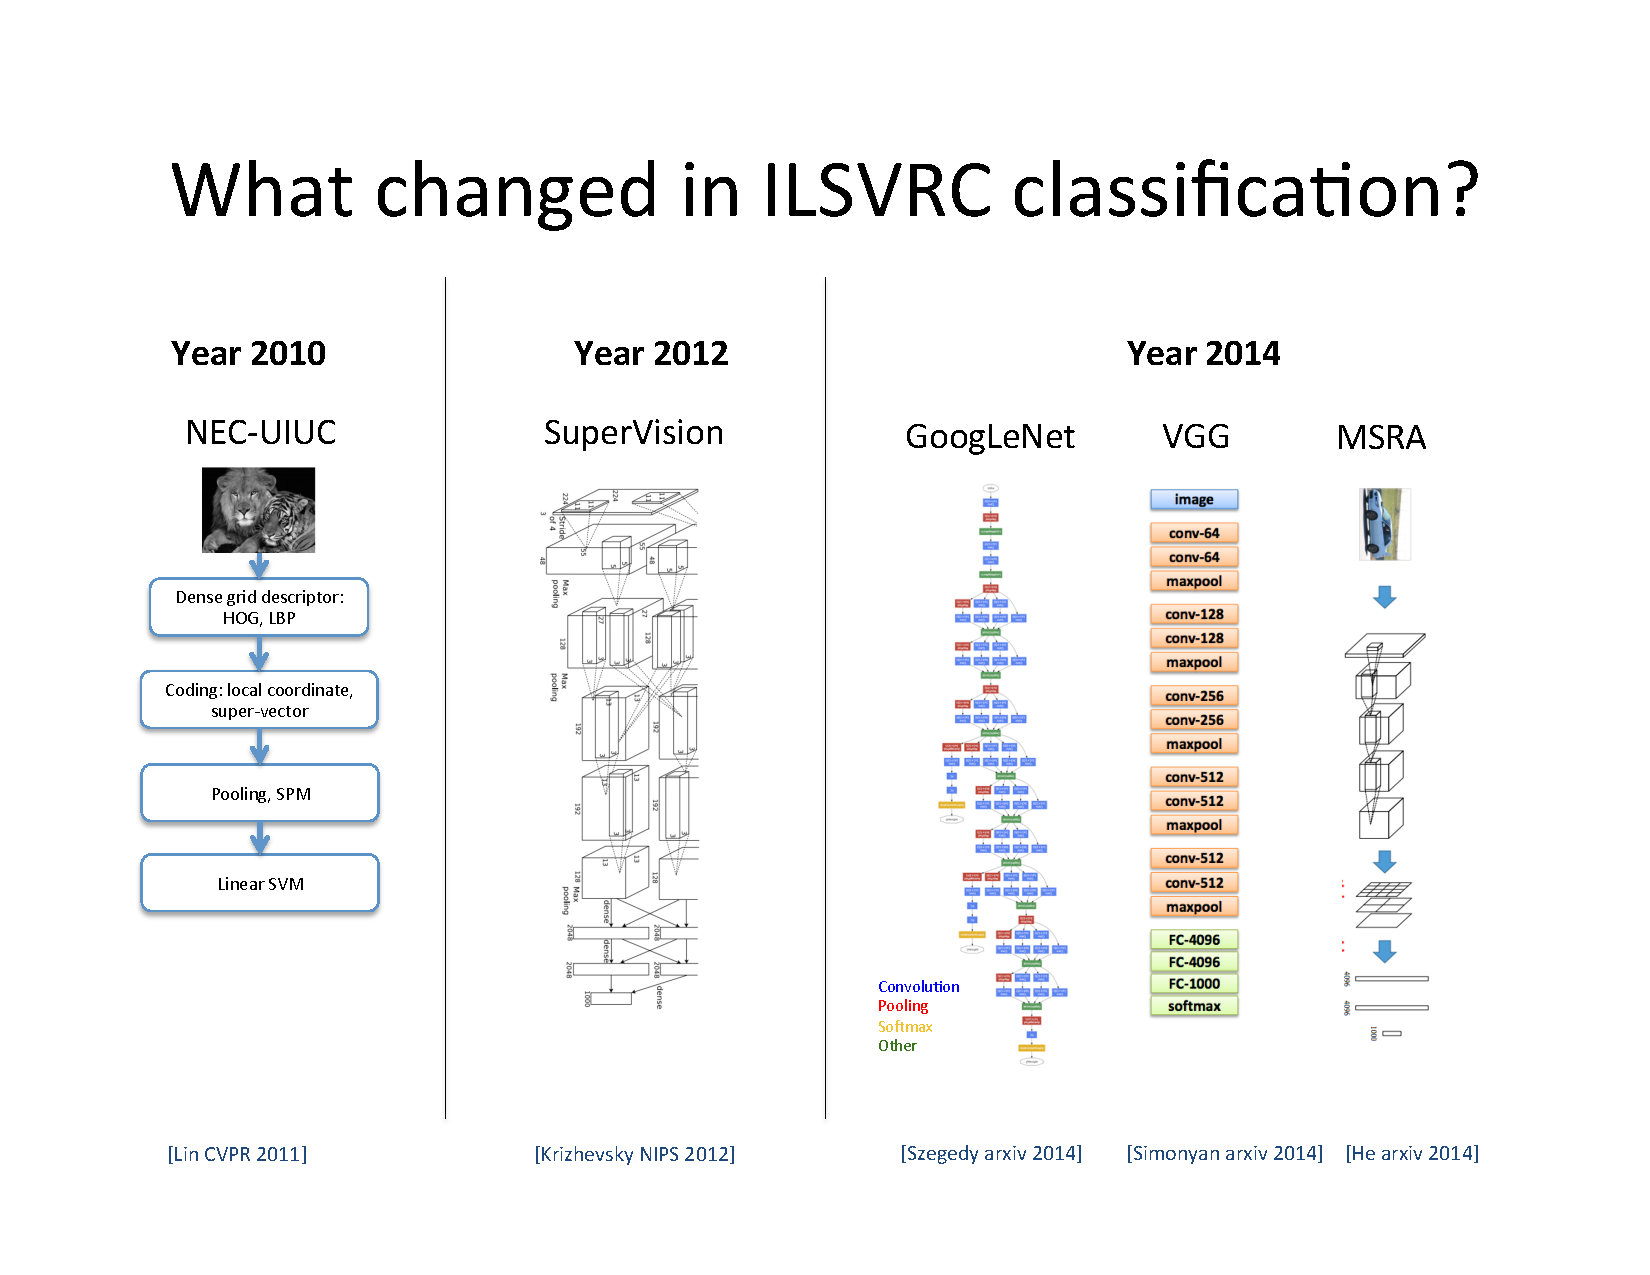
\includegraphics[width=0.8\linewidth]{figures/netsoverview.pdf}
            %\caption{}
        \end{figure}
	\end{frame}
	}

	\begin{frame}{Top-5 error rate over time}%********************
	\begin{center}
	\begin{table}
	\begin{tabular}{ c c c c } 
	 Year & Team Name & Model & Error \\ 
	\hline
	\color{red}2012 & \color{red}SuperVision  & \color{red}AlexNet &  {\color{red} 16.42  } \\ 
	2013 & Clarifai     & ZF Net &  {\color{red} 11.74  } \\ 
	2014 & VGG         &  VGGNet &  {\color{red} 7.32  } \\ 
	2014 & GoogLeNet   & GoogLeNet &  {\color{red}  6.67  } \\ 
	2015 & MSRA          & ResNet &  {\color{red} 3.6  } \\  
	\end{tabular}
	\end{table}  
	\end{center}

	\head{AlexNet}
	\begin{itemize}
	\item The first work that popularized Convolutional Networks in Computer Vision
	\item The Network has a very similar architecture to LeNet, but is deeper, bigger, and featured Convolutional Layers stacked on top of each other.
	\end{itemize} 
	\end{frame}
	
	
	\begin{frame}{AlexNet Architecture}%********************
	\begin{center}
	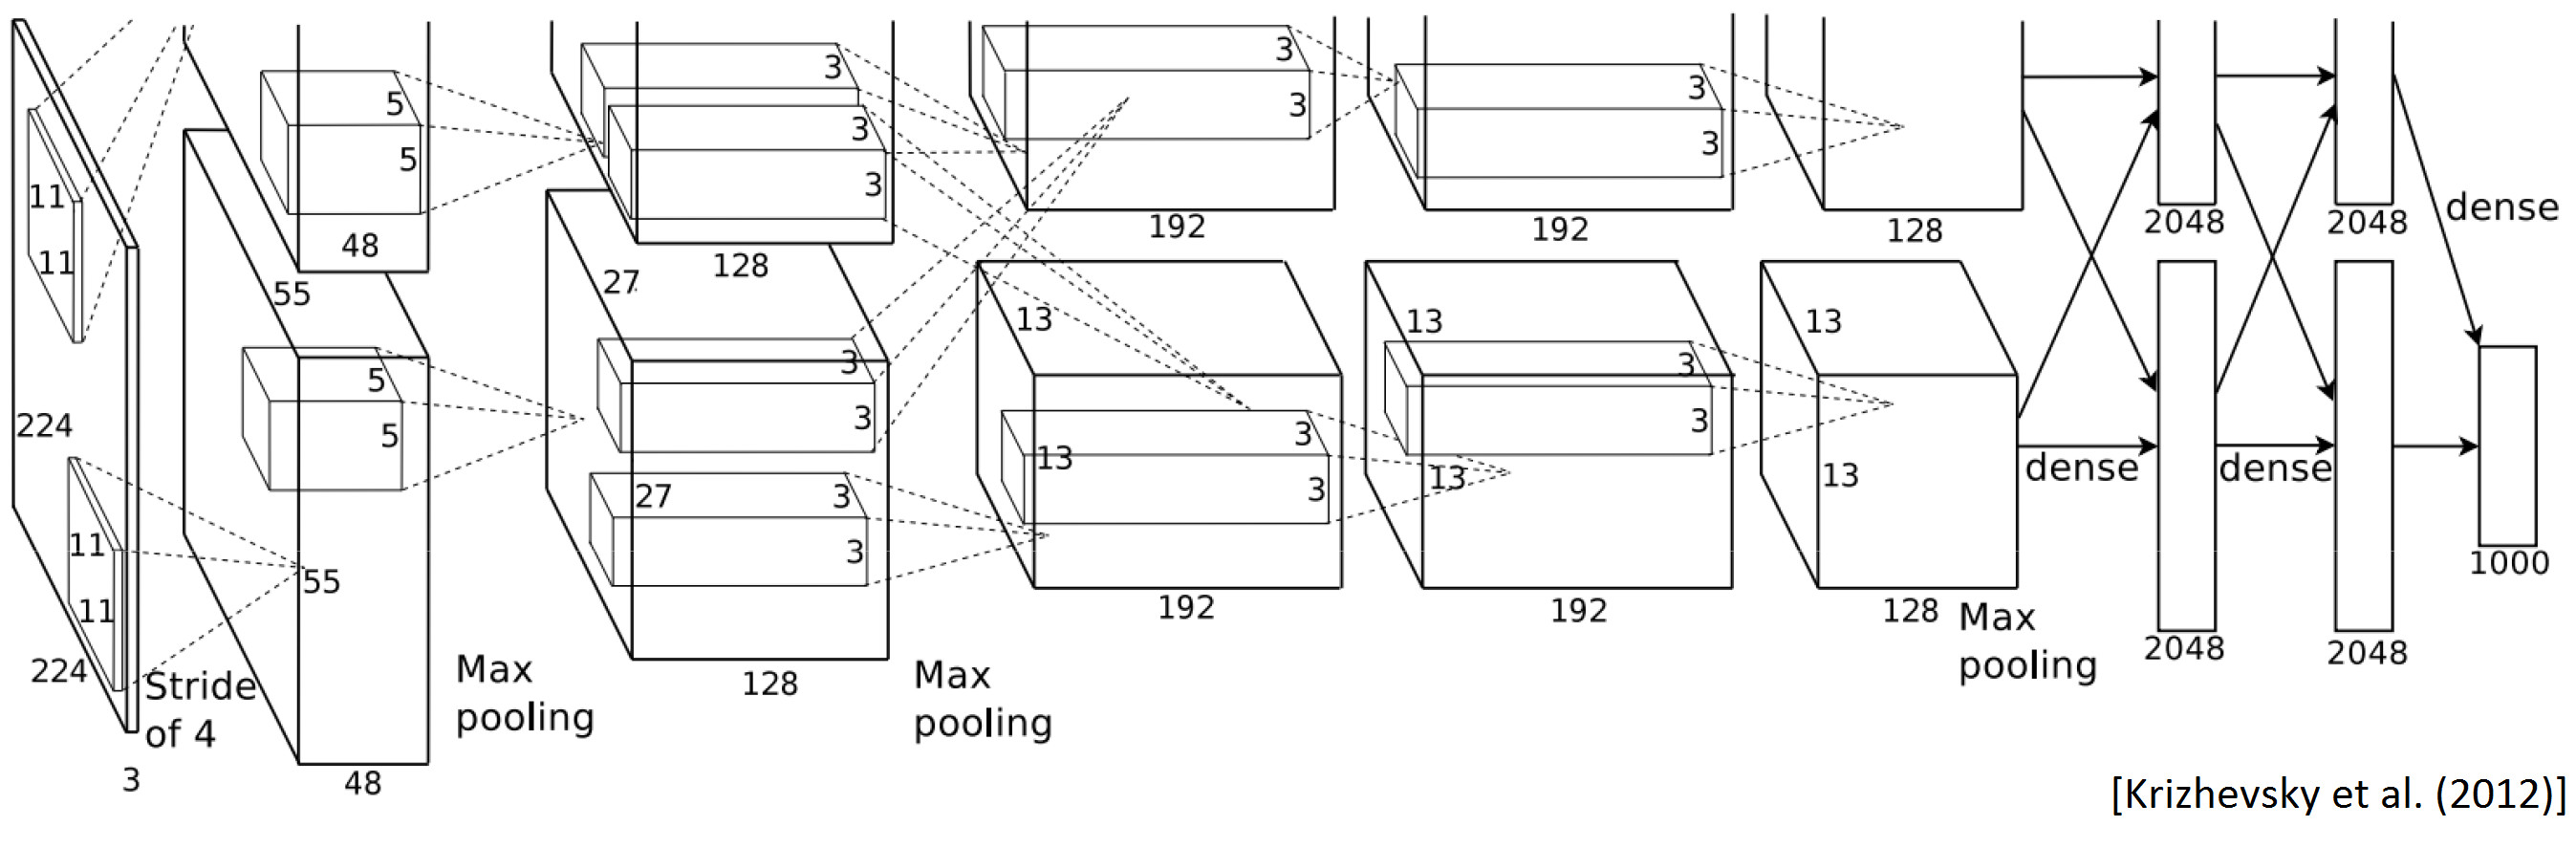
\includegraphics[scale=0.13]{figures/alexnet_paper.jpg} 
	\end{center}
	\footnotesize
	\begin{itemize}
	\item Trained with Stochastic Gradient Descent for six days on two NVIDIA GTX 580 3GB GPUs.
	\item Has 650.000 neurons, 60 million parameters, 630 million connections
	\item Down-sampled the images to a fixed resolution of $256 \times256$
	\end{itemize} 
	\note{'All of our experiments suggest that our results can be improved simply by waiting for faster GPUs and bigger datasets to become available'; a convolutional layer with N filters can be run on two GPUs, each of which convolves its input with N/2 filters}
	\end{frame}
	
		{ \referencefootnote{\href{http://image-net.org/challenges/LSVRC/2012/supervision.pdf}{Slide from \underline{here}.}}
	\begin{frame}{Validation classification}%********************
				\begin{figure}
            \centering
            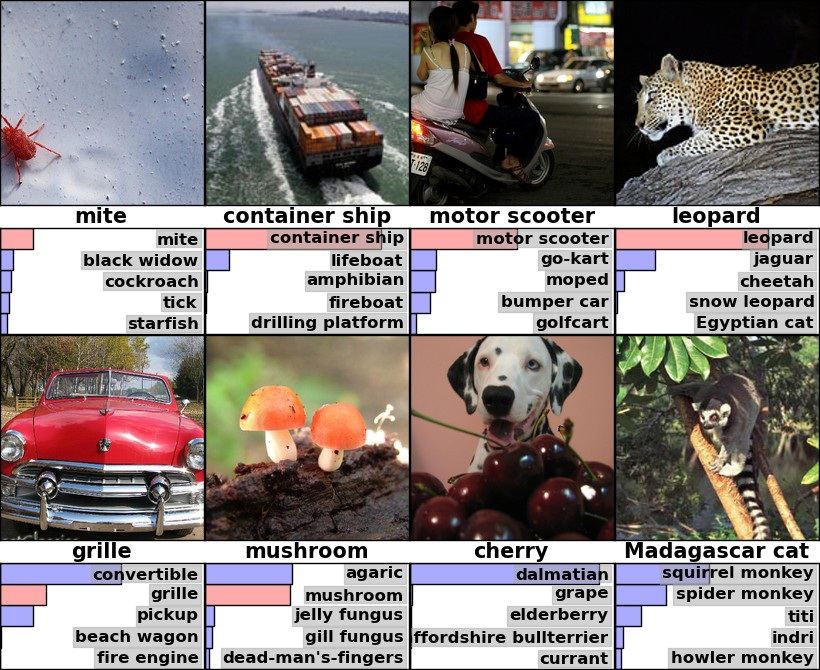
\includegraphics[width=0.7\linewidth]{figures/alexnet_validation.jpg}
            %\caption{}
        \end{figure}
	\end{frame}
	}
	
	{ \referencefootnote{\href{http://cs231n.stanford.edu/slides/2017/cs231n_2017_lecture12.pdf}{Slide from \underline{here}.}}
		\begin{frame}{Visualization: Last Layer} %******************** 
						\begin{figure}
            \centering
            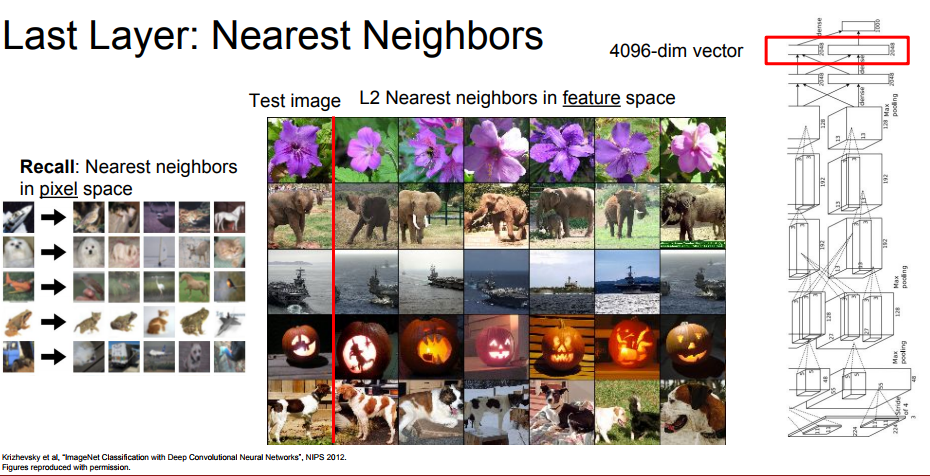
\includegraphics[width=0.9\linewidth]{figures/Selection_019.png}
            %\caption{}
        \end{figure}
	\end{frame}
	}
	
	\begin{frame}{Top-5 error rate over time}%********************
	\begin{center}
	\begin{table}
	\begin{tabular}{  c   c  c  c   c  } 
	 Year & Team Name & Model & Error \\ 
	\hline
	 2012 &  SuperVision  &  AlexNet &  { \color{red} 16.42  }  \\ 
	2013 & Clarifai     & ZF Net&  {\color{red} 11.74  }  \\ 
	\color{red}2014 & \color{red}VGGNet         &  \color{red}VGG &  {\color{red} 7.32  } \\ 
	2014 & GoogLeNet   & GoogLeNet &  {\color{red}  6.67  } \\ 
	2015 & MSRA          & ResNet &  {\color{red} 3.6  } \\  
	\end{tabular}
	\end{table}  
	\end{center}
	\footnotesize
	VGGNet
	\begin{itemize}
	\item  Main contribution: Depth matters!, from 11 to 19 weight layers.
	\item Extremely homogeneous architecture by using smaller-size convolution filters: only 3x3 convolutions and 2x2 pooling throughout the whole net.
	\item Expensive to evaluate and requires more memory 
	\end{itemize}
	\end{frame} 

	 
		
	% \subsection{VGGNet Architecture} 

	\begin{frame}{VGGNet Architecture}%********************
			\begin{figure}
            \centering
            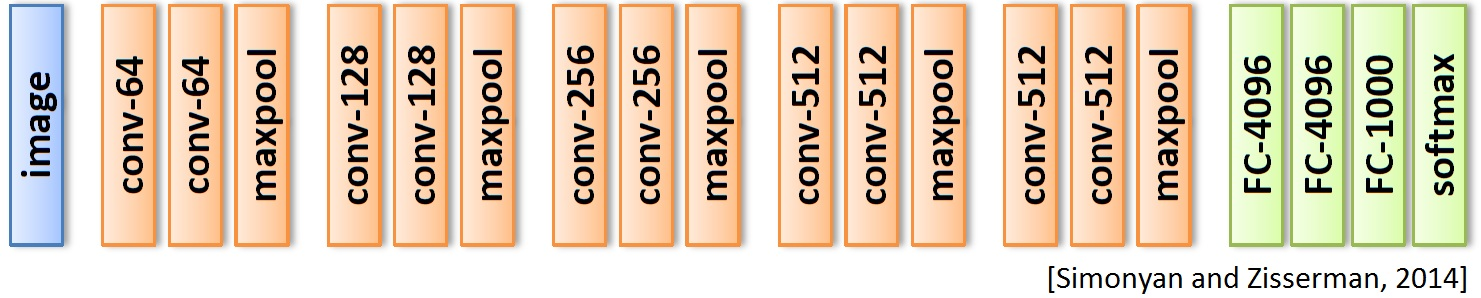
\includegraphics[width=0.8\linewidth]{figures/vggnet_single.jpg}
            %\caption{}
        \end{figure}
	\footnotesize
	Key design choices :  
	\begin{itemize}
	\item Convolutional layers
	\begin{itemize}
	\item  $3\times3$ conv. filters - the smallest size to capture the notion of left/right, up/down, center
	\item  Stride 1 – no loss of information, with  1 pixel padding
	\end{itemize}
	\item Max-pooling
	\begin{itemize}
	\item  performed over a  $2\times2$ pixel window, with stride 2
	\item 5 max-pool layers (x2 reduction)
	\end{itemize}  
	\item 3 fully-connected (FC) layers 
	\end{itemize}   
	\end{frame}

\begin{frame}{Top-5 error rate over time}%********************
	\begin{center}
	\begin{table}
	\begin{tabular}{  c   c  c  c   c  } 
	 Year & Team Name & Model & Error\\ 
	\hline
	 2012 &  SuperVision  &  AlexNet &  { \color{red} 16.42  }  \\ 
	2013 & Clarifai     & ZF Net&  {\color{red} 11.74  }  \\ 
	 2014 & VGGNet         &  VGG &  {\color{red} 7.32  }  \\ 
	 2014 & GoogLeNet   &  GoogLeNet &  {\color{red}  6.67 } \\ 
	\color{red}2015 & \color{red}MSRA          & \color{red}ResNet &  {\color{red} 3.6  } \\  
	\end{tabular}
	\end{table}  
	\end{center}

	ResNet
	\begin{itemize}
	\item  Revolution of Depth
	\end{itemize} 
	\end{frame} 
	
		\begin{frame}{Revolution of Depth}%********************
	\begin{center}
	\captionfig{figures/resnet_revolution_depth.jpg}{0.9}{slide from \href{http://image-net.org/challenges/talks/ilsvrc2015_deep_residual_learning_kaiminghe.pdf}{[here]}} 
	\end{center} 
	\end{frame}
	
	\begin{frame}{Revolution of Depth}%********************
	\begin{center}
	\captionfig{figures/resnet_at_competitions.jpg}{1}{slide from \href{http://kaiminghe.com/icml16tutorial/icml2016_tutorial_deep_residual_networks_kaiminghe.pdf}{[here]}} 
	\end{center}
	\end{frame} 

{ \referencefootnote{\href{http://image-net.org/challenges/talks/ilsvrc2015_deep_residual_learning_kaiminghe.pdf}{Image from \underline{here}.}}
	\begin{frame}{Simply stacking layers?} %********************
	\begin{center}
	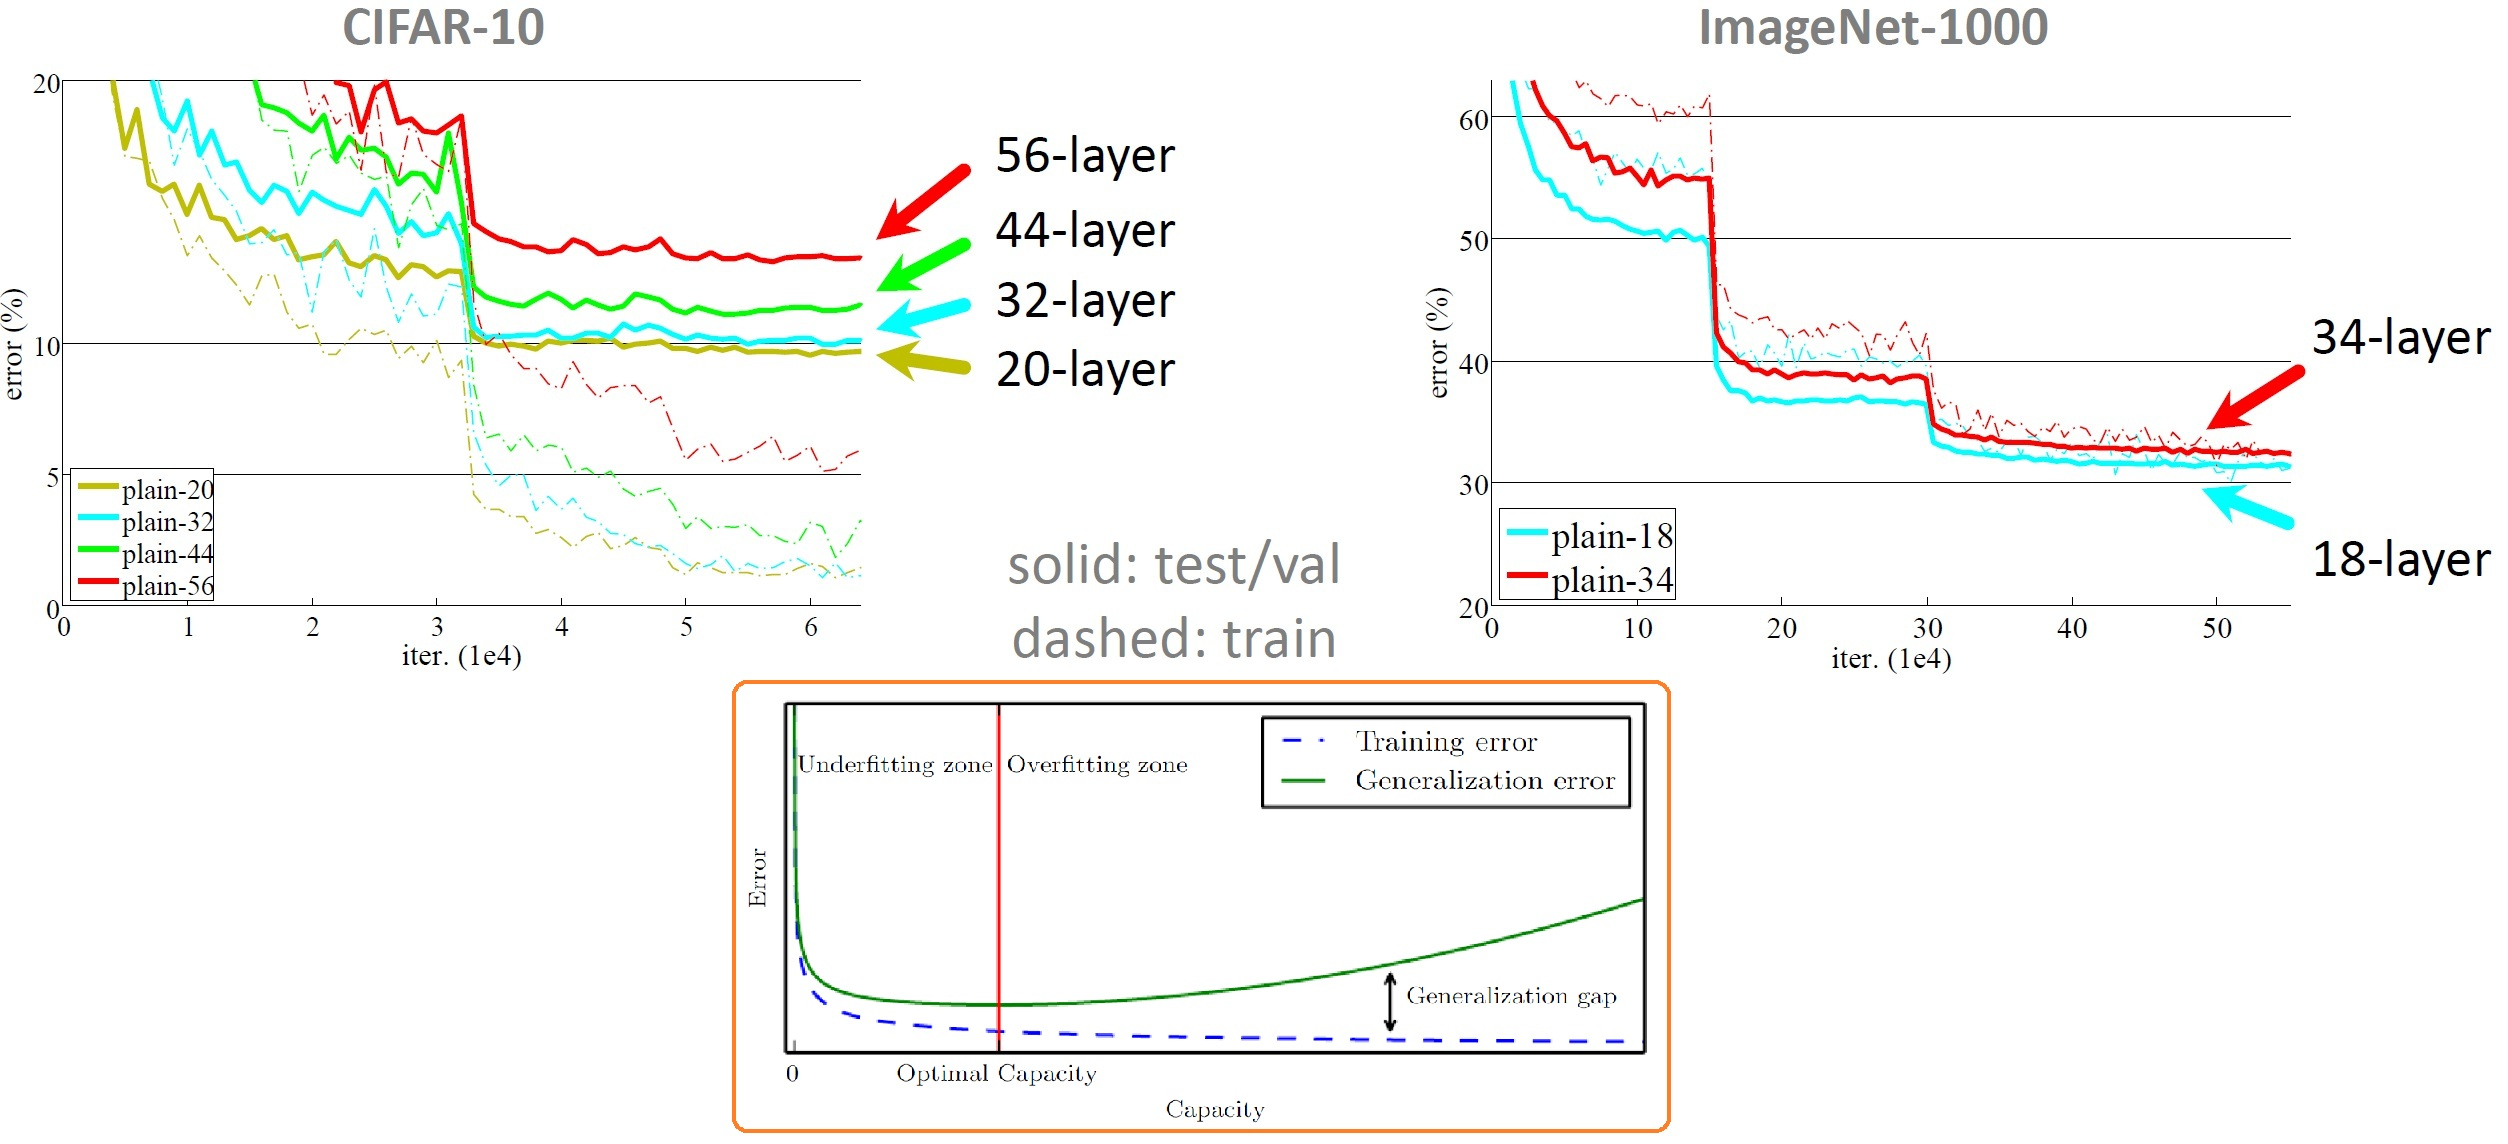
\includegraphics[scale=0.15]{figures/resnet_stacking_layers.jpg}  
	%\captionfig{figures/resnet_stacking_layers.jpg}{0.9}{slide from \href{http://image-net.org/challenges/talks/ilsvrc2015_deep_residual_learning_kaiminghe.pdf}{[here]}}
	\end{center} 
	\footnotesize
	\begin{itemize}
	\item  Plain nets:	stacking $3 \times 3$ conv layers. 
	\item 'Overly deep' plain nets have higher training error
	\item A general phenomenon, observed in many datasets
	\end{itemize} 
	\note{if you stack multiple layers and train them you get a high error. And this is not in the test data it is not due to over fitting. It is in the training data. 56 layer model perform worse than 20 layer model, even though the 56 layer model has a bigger capacity.  The expectation is 56 layered model at least can imitate 20 layered model by setting to compute identities. This is an optimization problem, that you can't find the solution}
	\end{frame}
}

	% \subsection{ResNet Architecture} 

	\begin{frame}{ResNet Architecture} %********************
	\begin{center}
	\captionfig{figures/resnet_vgg_contruction.jpg}{0.9}{slide from \href{http://image-net.org/challenges/talks/ilsvrc2015_deep_residual_learning_kaiminghe.pdf}{[here]}} 
	\end{center} 
	\note{Deeper networks do not have less error. Difficulty lies in the optimization. SGD is not an ideal optimizer so in experiments researchers found that increased depth brought increased training error, which was not in line with the intuition nor 'theory'. The increased training error indicates that the ultra-deep network is very hard to optimize/train.}
	\end{frame}


	\begin{frame}{Network Design} %******************** 
	\begin{center}
	\captionfig{figures/resnet_keep_it_simple.jpg}{0.8}{slide from \href{http://image-net.org/challenges/talks/ilsvrc2015_deep_residual_learning_kaiminghe.pdf}{[here]}} 
	\end{center} 
	\note{Authors wired the layers in a such way you monotonically get a better performance as you add new layers into the network and you dont run into the optimization problems. 
	They follow the philosophy of the VGGnet, 3x3 convolutions, each time they reduce the spatial size with 2, and increase the number of filter by 2, by doing so time complexity of the network stays the same}
	\end{frame}

	\begin{frame}{Deep	Residual Learning (Residual Block)}%********************
	\begin{center}
	\captionfig{figures/resnet_plain_residual.jpg}{0.8}{slide from \href{http://image-net.org/challenges/talks/ilsvrc2015_deep_residual_learning_kaiminghe.pdf}{[here]}}
	\end{center} 
	\footnotesize
	\begin{itemize}  
	\item  Adding skip-connections (skipping one or more layers) that are summed with the output of the convolution layers.  
	\item Identity skip-connections don't add extra parameter or computational complexity.
	\end{itemize}
	\note{You have this pathway where you have this representation of the image x, and then instead of transforming that representation x to get a new x to plug in later, having this x  we are doing some compute on aside that is that residual block doing some computations and then you add your result on top of x. So you have this addition operation going to the next residual block. You have x and you are always computing deltas to it. In back propagation, addition operation is a gradient distributor, you  get a gradient from the top and this gradient will flow equally to all the children participated in that addition. You have gradient flow in here from the supervision, you have supervision here at the very bottom in this diagram and it flows upwards through, and it flows through these residual blocks than gets added to the stream. This addition distributes that gradient identically through.  You end up with a gradient super highway. The gradients from your supervision go directly to the original convolutional layers, and then on top of that you get these deltas from all these residual blocks, so these blocks can help out that original stream of information. Addition operation makes the gradient flow significantly better}
	\end{frame}
	
	\begin{frame}{CIFAR-10 experiments} %******************** 
	\begin{center}
	\captionfig{figures/resnet_cifar_plain_resnet.jpg}{1}{slide from \href{http://image-net.org/challenges/talks/ilsvrc2015_deep_residual_learning_kaiminghe.pdf}{[here]}}
	\end{center}  
	\begin{itemize}
	\item Deep ResNets can be trained without difficulties
	\item Deeper ResNets have lower training error, and also lower test error
	\end{itemize} 
	\end{frame}
	 
	     \begin{frame}{Summary}
        \begin{itemize}
            \item Deeper models tend to perform better.
            \item Skip-connections allow us to train very deep networks.
        \end{itemize}
    \end{frame}

    \begin{frame}[allowframebreaks]{Literature}
        \printbibliography
    \end{frame}
    
\end{document}
